\documentclass{beamer}
\usepackage[english,activeacute]{babel}
\usepackage[utf8]{inputenc}
\usepackage{listings}
\usepackage{color}
\usepackage{tikz}

\definecolor{red}{RGB}{255,0,0}
\definecolor{green}{RGB}{0,255,0}
\definecolor{blue}{RGB}{0,0,255}
\definecolor{oran}{RGB}{255,93,0}

\newcommand{\blue}{\textcolor{blue}}
\newcommand{\red}{\textcolor{red}}
\newcommand{\green}{\textcolor{green}}
\newcommand{\oran}{\textcolor{oran}}
\newcommand{\gray}{\textcolor{gray}}
\definecolor{gray97}{gray}{.97}
\definecolor{gray75}{gray}{.75}
\definecolor{gray45}{gray}{.45}

\renewcommand\mathfamilydefault{\rmdefault}
\setbeamertemplate{blocks}[rounded][shadow=true]

\usetheme[pageofpages=of,
          alternativetitlepage=true,
          titlepagelogo=img/aei,
          watermark=,
          watermarkheight=50px,
          watermarkheightmult=1,
          ]{Torino}

\lstset{ frame=Ltb,
     framerule=0pt,
     aboveskip=0.5cm,
     framextopmargin=3pt,
     framexbottommargin=3pt,
     framexleftmargin=0.4cm,
     framesep=0pt,
     rulesep=.4pt,
     backgroundcolor=\color{gray97},
     rulesepcolor=\color{black},
     %
     stringstyle=\ttfamily,
     showstringspaces = false,
     basicstyle=\tiny\ttfamily,
     %commentstyle=\color{gray45},
     %keywordstyle=\bfseries,
     %
     numbers=left,
     numbersep=13pt,
     numberstyle=\tiny,
     numberfirstline = false,
     breaklines=true,
     emph = {[1]\_\_device\_\_,\_\_global\_\_,\_\_syncthreads,pthread\_create,pthread\_join,pragma,omp,parallel,private, threadIdx, blockDim, blockIdx,cudaThreadSynchronize, while, total},
     emphstyle={[1]\color{blue}},
   }

% minimizar fragmentado de listados
\lstnewenvironment{listing}[1][]
   {\lstset{#1}\pagebreak[0]}{\pagebreak[0]}

\lstdefinestyle{consola}
   {basicstyle=\scriptsize\bf\ttfamily,
    backgroundcolor=\color{gray75},
   }
\lstdefinestyle{C}
   {language=C,
   }



\usecolortheme{nouvelle}
\vspace{-0.5cm}
\author[C. Maureira and P. Amaro-Seoane]
       {\large Cristián Maureira\\
        \large Pau Amaro-Seoane}
\title[GraviDy]
      {\huge \texttt{GraviDy}}
\subtitle{\large A modular direct $N$-body GPU integrator.}
\institute[AEI]
          {Albert Einstein Institute}

\begin{document}

\bibliographystyle{unsrt}
%\pagestyle{empty}

% First slide
\begin{frame}[t,plain]
    \titlepage
\end{frame}

\section{Introduction}

\begin{frame}
    \frametitle{Introduction}
    \framesubtitle{Motivation (1/2)}

    \begin{columns}
        \begin{column}{0.6\textwidth}
            \begin{itemize}
                \item Dynamical evolution of a dense stellar systems.
                      ({\nbody} Problem)
                \item Newtonian systems compounded by \blue{more than two stars},
                      needs numerical approaches.
            \end{itemize}
        \end{column}
        \begin{column}{0.4\textwidth}
            \begin{figure}
                \centering
                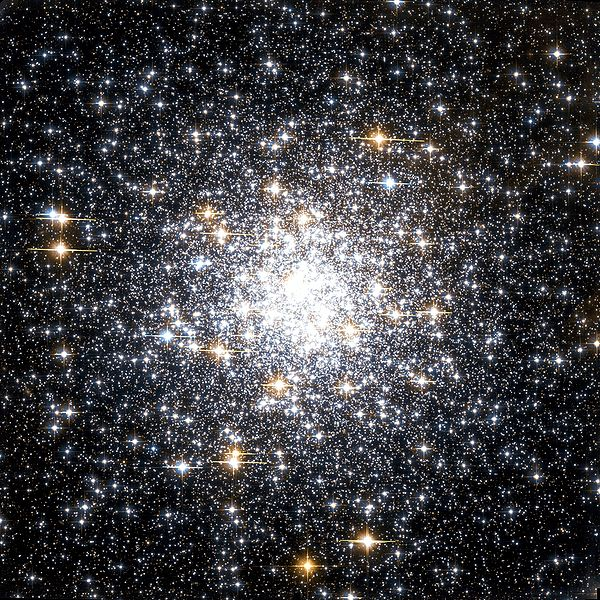
\includegraphics[width=0.8\textwidth]{img/m69}
                \caption{Globular cluster ``Messier 69'' in the constellation Sagittarius.}
                \label{fig:m69}
            \end{figure}
        \end{column}
    \end{columns}
\end{frame}

\begin{frame}
    \frametitle{Introduction}
    \framesubtitle{Motivation (2/2)}

    \begin{columns}
        \begin{column}{0.5\textwidth}
            \begin{itemize}
                \item Evolution of the High Performance Computing (HPC).
            \end{itemize}
            \begin{center}
                
\includegraphics[width=0.8\textwidth]{img/top500}
            \end{center}
        \end{column}
        \begin{column}{0.5\textwidth}
            \begin{figure}
                \centering
                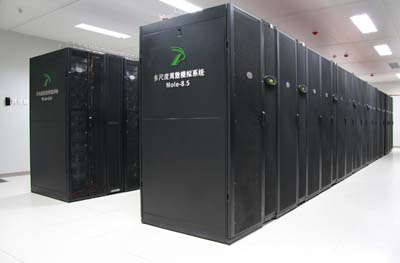
\includegraphics[width=0.8\textwidth]{img/cluster}
                \caption{GPU Cluster Mole-8.5 in Beijing, at the Institute of Process
                         Engineering of Chinese Academy of Sciences.
                         (372 nodes and 2,000 NVIDIA Fermi C2050 GPUs)}
                \label{fig:m69}
            \end{figure}
        \end{column}
    \end{columns}
\end{frame}

\section{The {\nbody} problem}
\begin{frame}
    \frametitle{The {\nbody} problem}
    \framesubtitle{Definition}

    Purely dynamic problem, in which the bodies orbital evolution
    is determined exclusive by the \blue{gravitational interaction},

    \begin{align}
        \bs{\ddot{r}}_{i} &= -G \sum\limits^{N}_{\substack{j=1\\j\neq i}}
                              m_{j} {(\bs{r}_i - \bs{r}_j)\over
                              | \bs{r}_i - \bs{r}_j|^{3}}\label{eq:nbody},
    \end{align}

    \noindent
    where $G$ is the gravitational constant
    ($6.67384\times 10^{-11} m^{3} kg^{-1} s^{-2}$),
    $m_j$ is the mass of the $j$th particle
    and $\bs{r}_j$ the position in \emph{Cartesian} coordinates.
    \begin{block}{\red{Note}}
        We denote vectors by bold fonts.
    \end{block}
\end{frame}


\begin{frame}
    \frametitle{The {\nbody} problem}
    \framesubtitle{Checking the system evolution}

    \begin{itemize}
        \item The \blue{initial condition} are usually the masses,
            position and velocity.

        \item \blue{Chaotic nature}, the evolution of this systems
         will depend of the initial parameters.

        \item The often invariant to check the integration of the system,
            is the system's \blue{energy},

            \begin{align}
                E &= {1 \over 2} \sum\limits^{N}_{i=1} m_{i} \bs{v}_{i}^{2} -
                     \sum\limits_{i=1}^{N} \sum\limits_{j > i}^{N}
                     {G m_{i} m_{j} \over |\bs{r}_{i} - \bs{r}_{j}|},
            \end{align}

            \noindent
            where $\bs{v}_i$ is the velocity of the particle $i$.
    \end{itemize}

\end{frame}


\begin{frame}
    \frametitle{The {\nbody} problem}
    \framesubtitle{Particle's time steps}

    \begin{itemize}
        \item The real scenario, \blue{individual} time steps.
        \begin{itemize}
            \item \red{Hard} scenario for parallel computing.
        \end{itemize}
        \item Forming groups of particles, \blue{block} time steps scheme~\cite{Press86}.
        \begin{itemize}
            \item  This time step scheme is popular among  {\nbody} code,
                like Starlab~\cite{portegies2001, hut2003}, Aarseth {\nbody}
                codes~\cite{Aarseth99, Aarseth03,NitadoriAarseth2012},
                $\phi$GRAPE~\cite{harfst2008},
                which gives us the possibility to check our algorithm behavior.
        \end{itemize}
    \end{itemize}
\end{frame}


\begin{frame}
    \frametitle{Introduction}
    \framesubtitle{{\nbody} algorithms classification}

    \begin{description}
        \item[Collision-less]
            A star just sees the \blue{background potential} of the rest of
            the stellar system.
            A model of this situation is the Barnes-Hut Treecode
            with a complexity $O(N\log N)$~\cite{BarnesHut86}
            or the fast multipole method with $O(N)$~\cite{GreendardThesis}.
            \vspace{0.7cm}
        \item[Collisional (``direct-summation'')]
            One star integrates \blue{all gravitational forces}
            for all stars. This typically scale as $O(N^{2})$.
            A well-known example is the family of algorithm of Aarseth
            the direct-summation {\sc Nbody} integrator~\cite{Aarseth99,Spurzem1999,Aarseth03}
            or {\sc kira} code~\cite{PortegiesZwartEtAl01}.
    \end{description}

\end{frame}

\section{Computational aspects}
\begin{frame}
    \frametitle{Introduction}
    \framesubtitle{The computational challenge}

    \begin{itemize}
        \item The {\nbody} codes evolution is related to the available
                \blue{hardware} in our time.
        \item The algorithms with a complexity of $O(N^{2})$ or $O(N^{3})$ require
                \red{supercomputers}.
        \begin{itemize}
            \item  e.g \blue{beowulf clusters},
                which require a parallelization of the code
                ({\sc Nbody6++} developed by Spurzem et al.~\cite{Spurzem1999}).

            \item Special-purpose hardware, like the \blue{GRAPE} (short for GRAvity
                PipE system~\cite{TMFES96,MT98,Makino98,GRAPE6A}.

        \end{itemize}

        \item  The literature overview reveals a strong interest on porting the existing codes to the
            \blue{GPU} architecture, like e.g. the work
            of~\cite{Portegies2007a,Hamada2007,Belleman2008}
            on single nodes or using large
            clusters~\cite{berczik2011high,NitadoriAarseth2012,Capuzzo-DolcettaEtAl2013}.

    \end{itemize}

\end{frame}

\subsection{GPU Computing}
\begin{frame}
    \frametitle{Introduction}
    \framesubtitle{GPU Computing}

    \begin{columns}
        \begin{column}{0.6\textwidth}
            \begin{itemize}
                \item \emph{``Using a GPU (Graphic Processing Unit) together with
                      a CPU to accelerate scientific calculation operations
                      or general purpose calculation''}
            \end{itemize}
        \end{column}
        \begin{column}{0.4\textwidth}
             \begin{figure}
                 \centering
                 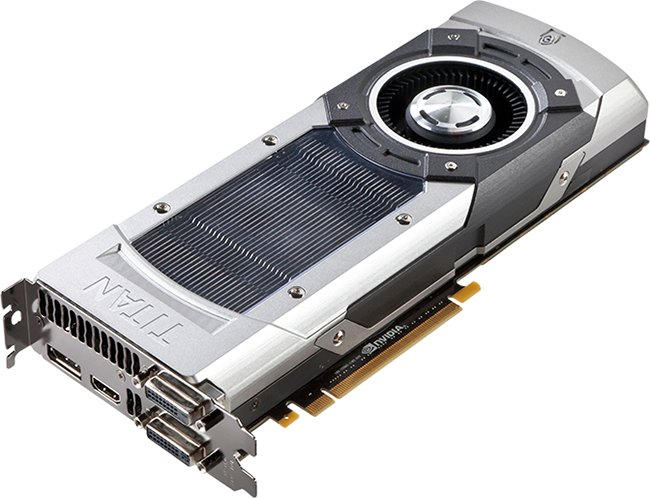
\includegraphics[width=0.8\textwidth]{img/titan}
                 \caption{NVIDIA\textsuperscript{\textregistered} GTX Titan}
                 \label{fig:titan}
             \end{figure}
        \end{column}
    \end{columns}
\end{frame}

\begin{frame}
    \frametitle{Introduction}
    \framesubtitle{CPU/GPU Design}

    \begin{itemize}
        \item CPU,
        \begin{itemize}
            \item Designed to have a good \blue{performance}
                  in parallel and non-parallel scenarios.
            \item Minimizes the \blue{latency} experimented by a thread
                  (large cache memory)
        \end{itemize}
        \item GPU,
            \begin{itemize}
            \item Designed to perform highly parallel work.
            \item Maximizes the \blue{throughput} of all the threads.
            \end{itemize}
    \end{itemize}

    \begin{footnotesize}
        \begin{columns}
            \begin{column}{0.35\textwidth}
            \begin{block}{Performance}
                Capacity of perform individual instructions in a certain time.
            \end{block}
            \end{column}
            \begin{column}{0.3\textwidth}
            \begin{block}{Latency}
                Measure of time delay experienced in a system.
            \end{block}
            \end{column}
            \begin{column}{0.3\textwidth}
            \begin{block}{Throughput}
                Capacity of perform a whole task in a certain time.
            \end{block}
            \end{column}
        \end{columns}
    \end{footnotesize}

    %\begin{description}
    %    \item[Performance]
    %            Capacity of perform individual instructions in a certain time.
    %    \item[Throughput]
    %            Capacity of perform a whole task in a certain time.
    %    \item[Latency]
    %            Measure of time delay experienced in a system.
    %    \item[Granularity]
    %            Break down a system into small parts.(Coarse and Fine)
    %\end{description}
\end{frame}

\begin{frame}
    \framesubtitle{Introduction}
    \frametitle{GPU Architecture}

    \begin{columns}
        \begin{column}{0.5\textwidth}
            \begin{block}{Task parallelism}
                Each processor perform a different task.
            \end{block}
            \begin{block}{Data parallelism}
                Each processor perform the same task, but not on the same data set.
            \end{block}
        \end{column}
        \begin{column}{0.5\textwidth}
             \begin{figure}
                 \centering
                 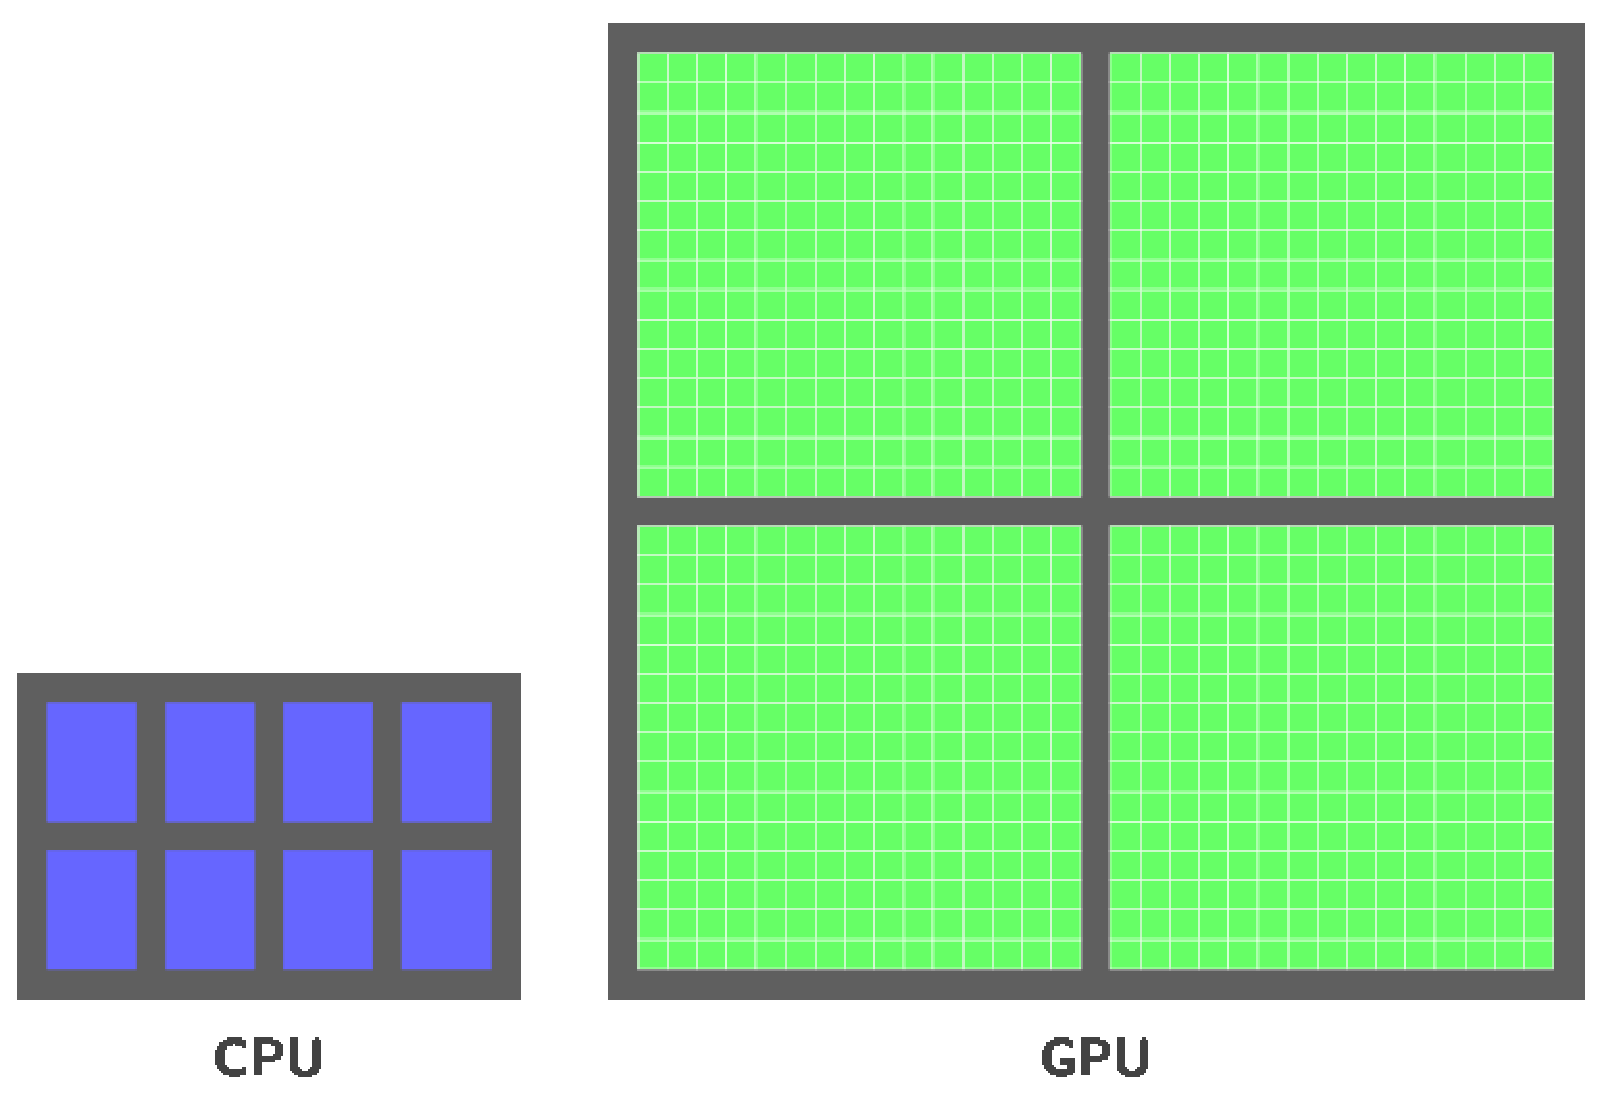
\includegraphics[width=0.8\textwidth]{img/cpu_gpu}
                 \caption{GPU and CPU core scheme}
                 \label{fig:titan}
             \end{figure}
        \end{column}
    \end{columns}
\end{frame}

\subsection{Programming strategy}
\begin{frame}
    \frametitle{Introduction}
    \framesubtitle{Programming strategy}

    \begin{columns}
        \begin{column}{0.5\textwidth}
            \begin{figure}
                \captionsetup{singlelinecheck=off}
                \centering
                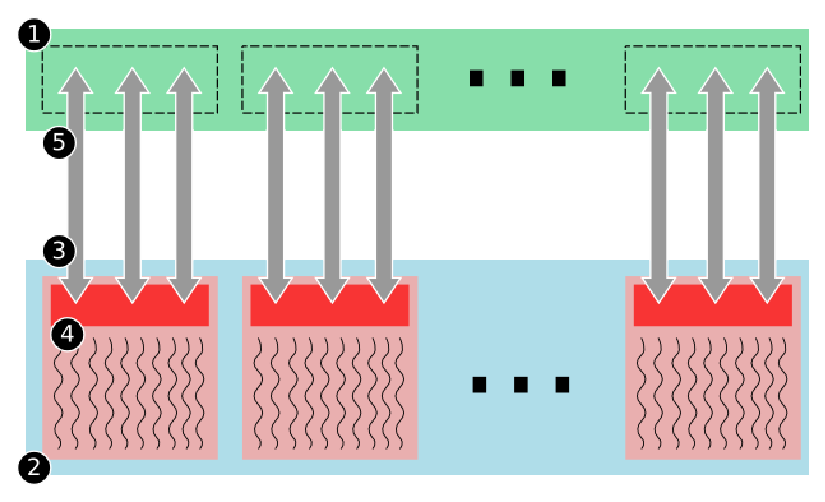
\includegraphics[width=0.9\textwidth]{img/cuda-strategy}
                \label{fig:estrategia}
                \caption{CUDA Programming strategy}
            \end{figure}
        \end{column}
        \begin{column}{0.5\textwidth}
             \begin{enumerate}
                 \item CPU memory allocation,
                 \item \dgreen{GPU} memory allocation,
                 \item Data copying,  CPU $\rightarrow$ \dgreen{GPU},
                 \item Task execution on the data,
                 \item Data copying, \dgreen{GPU} $\rightarrow$ CPU,
             \end{enumerate}
        \end{column}
    \end{columns}
\end{frame}

\begin{frame}
    \frametitle{GPU Computing}
    \framesubtitle{Introduction}

    \begin{columns}
        \begin{column}{0.5\textwidth}
            \begin{itemize}
                \item \emph{``Using a GPU (Graphic Processing Unit) together with
                      a CPU to accelerate scientific calculation operations
                      or general purpose calculation''}
            \end{itemize}
        \end{column}
        \begin{column}{0.5\textwidth}
             \begin{figure}
                 \centering
                 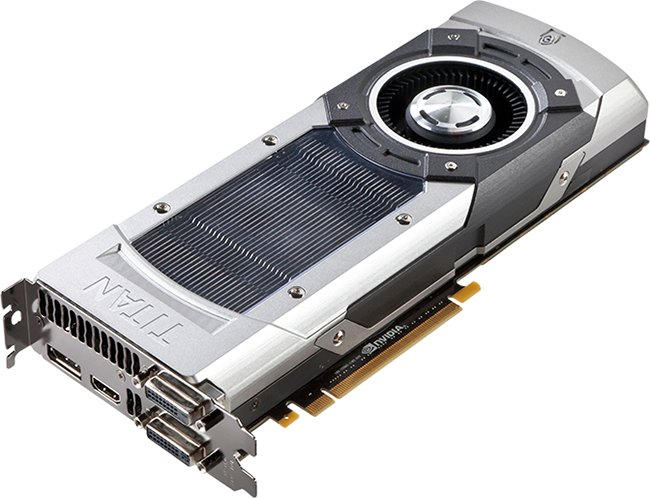
\includegraphics[width=0.8\textwidth]{img/titan}
                 \caption{NVIDIA\textsuperscript{\textregistered} GTX Titan}
                 \label{fig:titan}
             \end{figure}
        \end{column}
    \end{columns}
\end{frame}

\begin{frame}
    \frametitle{GPU Computing}
    \framesubtitle{Features}

    \begin{itemize}
        \item CPU,
        \begin{itemize}
            \item Designed to have a good \blue{performance}
                  in parallel and non-parallel scenarios.
            \item Minimizes the \blue{latency} experimented by a thread
                  (large cache memory)
        \end{itemize}
        \item GPU,
            \begin{itemize}
            \item Designed to perform highly parallel work.
            \item Maximizes the \blue{throughput} of all the threads.
            \end{itemize}
    \end{itemize}

    \begin{footnotesize}
        \begin{columns}
            \begin{column}{0.35\textwidth}
            \begin{block}{Performance}
                Capacity of perform individual instructions in a certain time.
            \end{block}
            \end{column}
            \begin{column}{0.3\textwidth}
            \begin{block}{Latency}
                Measure of time delay experienced in a system.
            \end{block}
            \end{column}
            \begin{column}{0.3\textwidth}
            \begin{block}{Throughput}
                Capacity of perform a whole task in a certain time.
            \end{block}
            \end{column}
        \end{columns}
    \end{footnotesize}

    %\begin{description}
    %    \item[Performance]
    %            Capacity of perform individual instructions in a certain time.
    %    \item[Throughput]
    %            Capacity of perform a whole task in a certain time.
    %    \item[Latency]
    %            Measure of time delay experienced in a system.
    %    \item[Granularity]
    %            Break down a system into small parts.(Coarse and Fine)
    %\end{description}
\end{frame}

\begin{frame}
    \frametitle{GPU Computing}
    \framesubtitle{Architecture}

    \begin{columns}
        \begin{column}{0.5\textwidth}
            \begin{block}{Task parallelism}
                Each processor perform a different task.
            \end{block}
            \begin{block}{Data parallelism}
                Each processor perform the same task, but not on the same data set.
            \end{block}
        \end{column}
        \begin{column}{0.5\textwidth}
             \begin{figure}
                 \centering
                 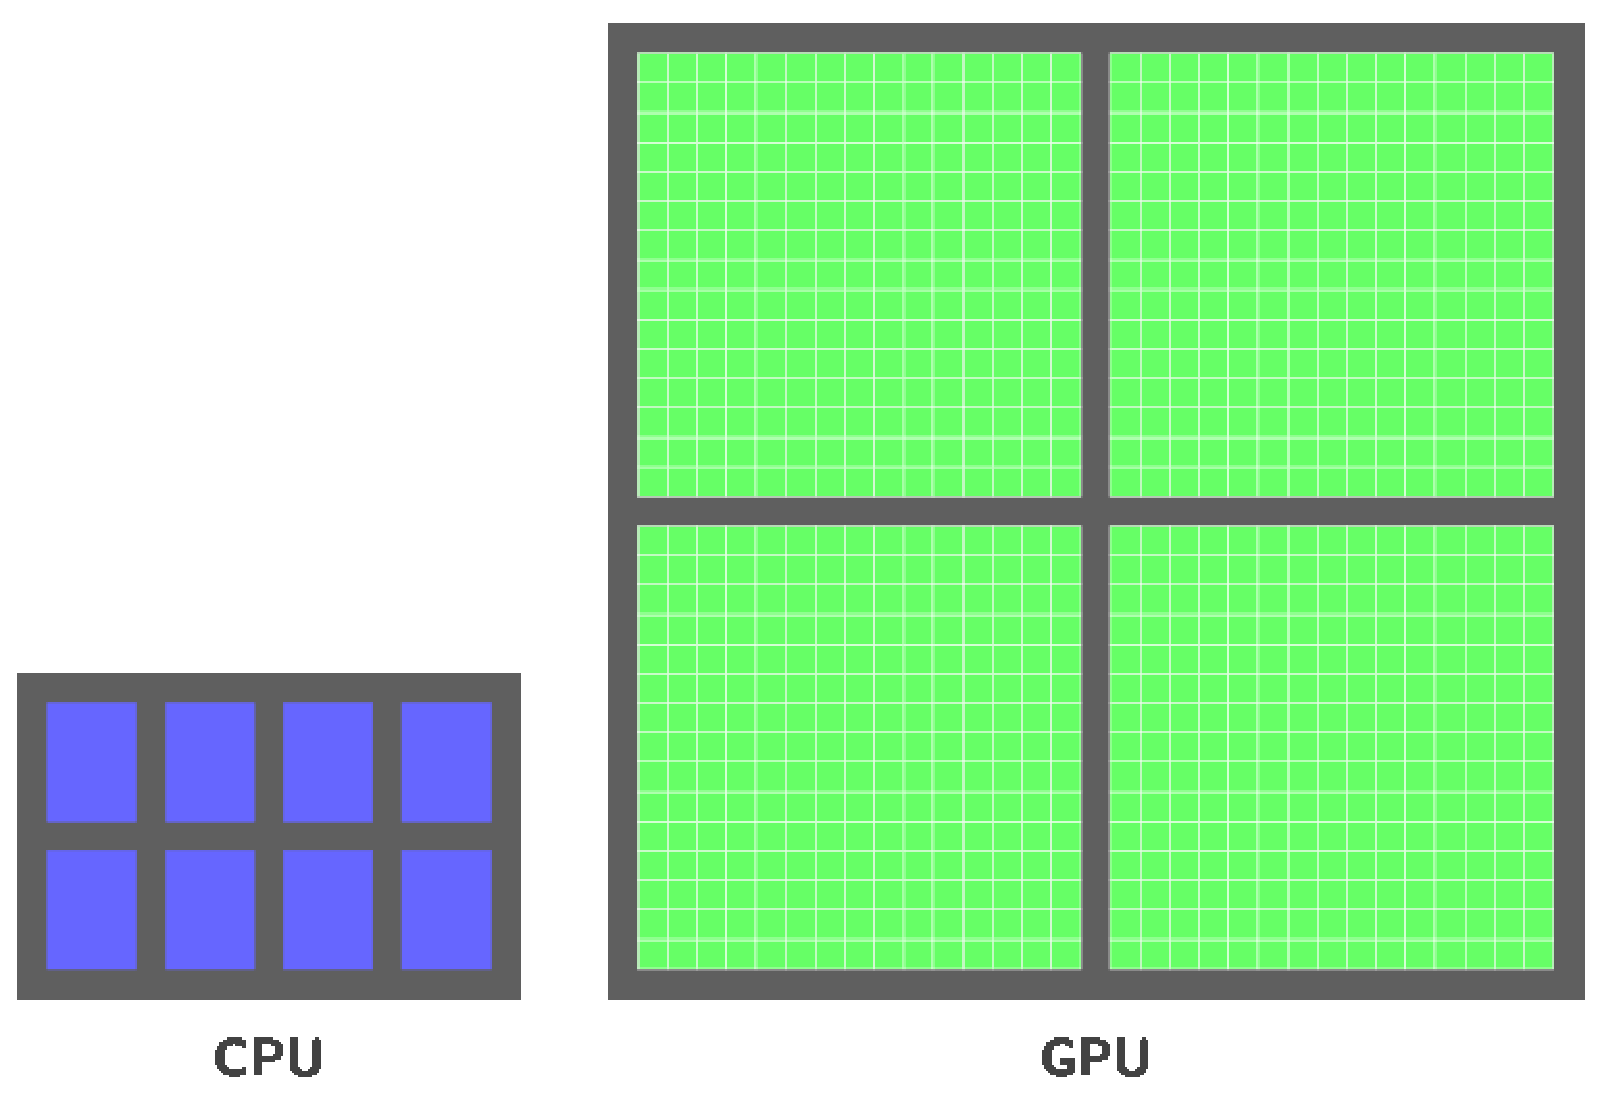
\includegraphics[width=0.8\textwidth]{img/cpu_gpu}
                 \caption{GPU and CPU core scheme}
                 \label{fig:titan}
             \end{figure}
        \end{column}
    \end{columns}
\end{frame}

\begin{frame}
    \frametitle{GPU Computing}
    \framesubtitle{Functionality}

    \begin{columns}
        \begin{column}{0.5\textwidth}
            \begin{figure}
                \captionsetup{singlelinecheck=off}
                \centering
                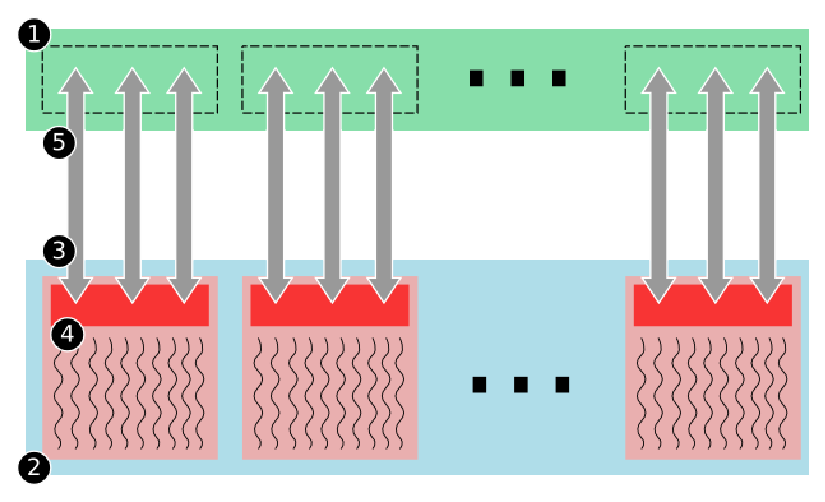
\includegraphics[width=0.9\textwidth]{img/cuda-strategy}
                \label{fig:estrategia}
                \caption{CUDA Programming strategy}
            \end{figure}
        \end{column}
        \begin{column}{0.5\textwidth}
             \begin{enumerate}
                 \item CPU memory allocation,
                 \item \dgreen{GPU} memory allocation,
                 \item Data copying,  CPU $\rightarrow$ \dgreen{GPU},
                 \item Task execution on the data,
                 \item Data copying, \dgreen{GPU} $\rightarrow$ CPU,
             \end{enumerate}
        \end{column}
    \end{columns}
\end{frame}


\documentclass{beamer}
\usepackage[english,activeacute]{babel}
\usepackage[utf8]{inputenc}
\usepackage{listings}
\usepackage{color}
\usepackage{tikz}

\definecolor{red}{RGB}{255,0,0}
\definecolor{green}{RGB}{0,255,0}
\definecolor{blue}{RGB}{0,0,255}
\definecolor{oran}{RGB}{255,93,0}

\newcommand{\blue}{\textcolor{blue}}
\newcommand{\red}{\textcolor{red}}
\newcommand{\green}{\textcolor{green}}
\newcommand{\oran}{\textcolor{oran}}
\newcommand{\gray}{\textcolor{gray}}
\definecolor{gray97}{gray}{.97}
\definecolor{gray75}{gray}{.75}
\definecolor{gray45}{gray}{.45}

\renewcommand\mathfamilydefault{\rmdefault}
\setbeamertemplate{blocks}[rounded][shadow=true]

%\usetheme[pageofpages=of,
%          alternativetitlepage=true,
%          titlepagelogo=img/aei,
%          watermark=,
%          watermarkheight=50px,
%          watermarkheightmult=1]{Torino}

\lstset{ frame=Ltb,
     framerule=0pt,
     aboveskip=0.5cm,
     framextopmargin=3pt,
     framexbottommargin=3pt,
     framexleftmargin=0.4cm,
     framesep=0pt,
     rulesep=.4pt,
     backgroundcolor=\color{gray97},
     rulesepcolor=\color{black},
     %
     stringstyle=\ttfamily,
     showstringspaces = false,
     basicstyle=\tiny\ttfamily,
     %commentstyle=\color{gray45},
     %keywordstyle=\bfseries,
     %
     numbers=left,
     numbersep=13pt,
     numberstyle=\tiny,
     numberfirstline = false,
     breaklines=true,
     emph = {[1]\_\_device\_\_,\_\_global\_\_,\_\_syncthreads,pthread\_create,pthread\_join,pragma,omp,parallel,private, threadIdx, blockDim, blockIdx,cudaThreadSynchronize, while, total},
     emphstyle={[1]\color{blue}},
   }

% minimizar fragmentado de listados
\lstnewenvironment{listing}[1][]
   {\lstset{#1}\pagebreak[0]}{\pagebreak[0]}

\lstdefinestyle{consola}
   {basicstyle=\scriptsize\bf\ttfamily,
    backgroundcolor=\color{gray75},
   }
\lstdefinestyle{C}
   {language=C,
   }



%\usecolortheme{nouvelle}
\vspace{-0.5cm}
\author[C. Maureira and P. Amaro-Seoane]
       {\large Cristián Maureira\\
        \large Pau Amaro-Seoane}
\title[GraviDy]
      {\huge \texttt{GraviDy}}
\subtitle{\large A modular direct $N$-body GPU integrator.}
\institute[AEI]
          {Albert Einstein Institute}

\begin{document}

\bibliographystyle{unsrt}
%\pagestyle{empty}

% First slide
\begin{frame}[t,plain]
    \titlepage
\end{frame}

\section{Introduction}

\begin{frame}
    \frametitle{Introduction}
    \framesubtitle{Motivation (1/2)}

    \begin{columns}
        \begin{column}{0.6\textwidth}
            \begin{itemize}
                \item Dynamical evolution of a dense stellar systems.
                      ({\nbody} Problem)
                \item Newtonian systems compounded by \blue{more than two stars},
                      needs numerical approaches.
            \end{itemize}
        \end{column}
        \begin{column}{0.4\textwidth}
            \begin{figure}
                \centering
                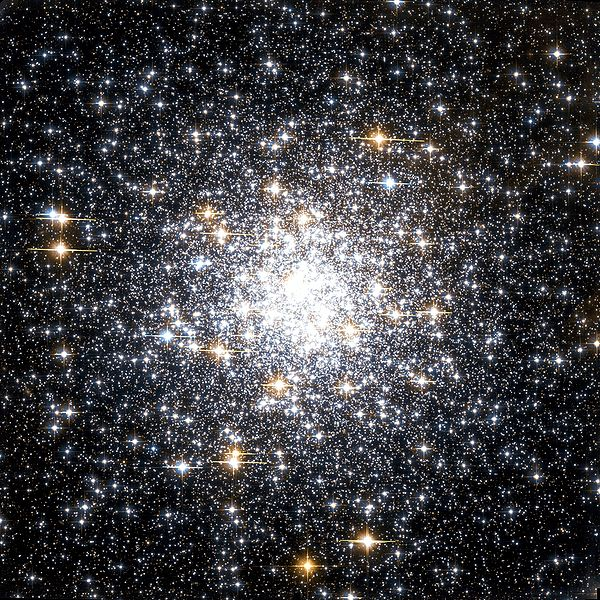
\includegraphics[width=0.8\textwidth]{img/m69}
                \caption{Globular cluster ``Messier 69'' in the constellation Sagittarius.}
                \label{fig:m69}
            \end{figure}
        \end{column}
    \end{columns}
\end{frame}

\begin{frame}
    \frametitle{Introduction}
    \framesubtitle{Motivation (2/2)}

    \begin{columns}
        \begin{column}{0.5\textwidth}
            \begin{itemize}
                \item Evolution of the High Performance Computing (HPC).
            \end{itemize}
            \begin{center}
                
\includegraphics[width=0.8\textwidth]{img/top500}
            \end{center}
        \end{column}
        \begin{column}{0.5\textwidth}
            \begin{figure}
                \centering
                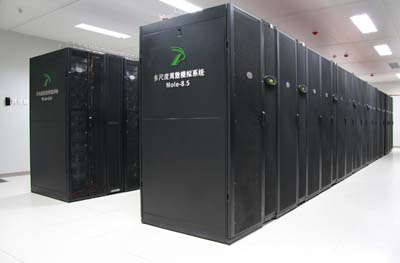
\includegraphics[width=0.8\textwidth]{img/cluster}
                \caption{GPU Cluster Mole-8.5 in Beijing, at the Institute of Process
                         Engineering of Chinese Academy of Sciences.
                         (372 nodes and 2,000 NVIDIA Fermi C2050 GPUs)}
                \label{fig:m69}
            \end{figure}
        \end{column}
    \end{columns}
\end{frame}

\section{The {\nbody} problem}
\begin{frame}
    \frametitle{The {\nbody} problem}
    \framesubtitle{Definition}

    Purely dynamic problem, in which the bodies orbital evolution
    is determined exclusive by the \blue{gravitational interaction},

    \begin{align}
        \bs{\ddot{r}}_{i} &= -G \sum\limits^{N}_{\substack{j=1\\j\neq i}}
                              m_{j} {(\bs{r}_i - \bs{r}_j)\over
                              | \bs{r}_i - \bs{r}_j|^{3}}\label{eq:nbody},
    \end{align}

    \noindent
    where $G$ is the gravitational constant
    ($6.67384\times 10^{-11} m^{3} kg^{-1} s^{-2}$),
    $m_j$ is the mass of the $j$th particle
    and $\bs{r}_j$ the position in \emph{Cartesian} coordinates.
    \begin{block}{\red{Note}}
        We denote vectors by bold fonts.
    \end{block}
\end{frame}


\begin{frame}
    \frametitle{The {\nbody} problem}
    \framesubtitle{Checking the system evolution}

    \begin{itemize}
        \item The \blue{initial condition} are usually the masses,
            position and velocity.

        \item \blue{Chaotic nature}, the evolution of this systems
         will depend of the initial parameters.

        \item The often invariant to check the integration of the system,
            is the system's \blue{energy},

            \begin{align}
                E &= {1 \over 2} \sum\limits^{N}_{i=1} m_{i} \bs{v}_{i}^{2} -
                     \sum\limits_{i=1}^{N} \sum\limits_{j > i}^{N}
                     {G m_{i} m_{j} \over |\bs{r}_{i} - \bs{r}_{j}|},
            \end{align}

            \noindent
            where $\bs{v}_i$ is the velocity of the particle $i$.
    \end{itemize}

\end{frame}


\begin{frame}
    \frametitle{The {\nbody} problem}
    \framesubtitle{Particle's time steps}

    \begin{itemize}
        \item The real scenario, \blue{individual} time steps.
        \begin{itemize}
            \item \red{Hard} scenario for parallel computing.
        \end{itemize}
        \item Forming groups of particles, \blue{block} time steps scheme~\cite{Press86}.
        \begin{itemize}
            \item  This time step scheme is popular among  {\nbody} code,
                like Starlab~\cite{portegies2001, hut2003}, Aarseth {\nbody}
                codes~\cite{Aarseth99, Aarseth03,NitadoriAarseth2012},
                $\phi$GRAPE~\cite{harfst2008},
                which gives us the possibility to check our algorithm behavior.
        \end{itemize}
    \end{itemize}
\end{frame}


\begin{frame}
    \frametitle{Introduction}
    \framesubtitle{{\nbody} algorithms classification}

    \begin{description}
        \item[Collision-less]
            A star just sees the \blue{background potential} of the rest of
            the stellar system.
            A model of this situation is the Barnes-Hut Treecode
            with a complexity $O(N\log N)$~\cite{BarnesHut86}
            or the fast multipole method with $O(N)$~\cite{GreendardThesis}.
            \vspace{0.7cm}
        \item[Collisional (``direct-summation'')]
            One star integrates \blue{all gravitational forces}
            for all stars. This typically scale as $O(N^{2})$.
            A well-known example is the family of algorithm of Aarseth
            the direct-summation {\sc Nbody} integrator~\cite{Aarseth99,Spurzem1999,Aarseth03}
            or {\sc kira} code~\cite{PortegiesZwartEtAl01}.
    \end{description}

\end{frame}

\section{Computational aspects}
\begin{frame}
    \frametitle{Introduction}
    \framesubtitle{The computational challenge}

    \begin{itemize}
        \item The {\nbody} codes evolution is related to the available
                \blue{hardware} in our time.
        \item The algorithms with a complexity of $O(N^{2})$ or $O(N^{3})$ require
                \red{supercomputers}.
        \begin{itemize}
            \item  e.g \blue{beowulf clusters},
                which require a parallelization of the code
                ({\sc Nbody6++} developed by Spurzem et al.~\cite{Spurzem1999}).

            \item Special-purpose hardware, like the \blue{GRAPE} (short for GRAvity
                PipE system~\cite{TMFES96,MT98,Makino98,GRAPE6A}.

        \end{itemize}

        \item  The literature overview reveals a strong interest on porting the existing codes to the
            \blue{GPU} architecture, like e.g. the work
            of~\cite{Portegies2007a,Hamada2007,Belleman2008}
            on single nodes or using large
            clusters~\cite{berczik2011high,NitadoriAarseth2012,Capuzzo-DolcettaEtAl2013}.

    \end{itemize}

\end{frame}

\subsection{GPU Computing}
\begin{frame}
    \frametitle{Introduction}
    \framesubtitle{GPU Computing}

    \begin{columns}
        \begin{column}{0.6\textwidth}
            \begin{itemize}
                \item \emph{``Using a GPU (Graphic Processing Unit) together with
                      a CPU to accelerate scientific calculation operations
                      or general purpose calculation''}
            \end{itemize}
        \end{column}
        \begin{column}{0.4\textwidth}
             \begin{figure}
                 \centering
                 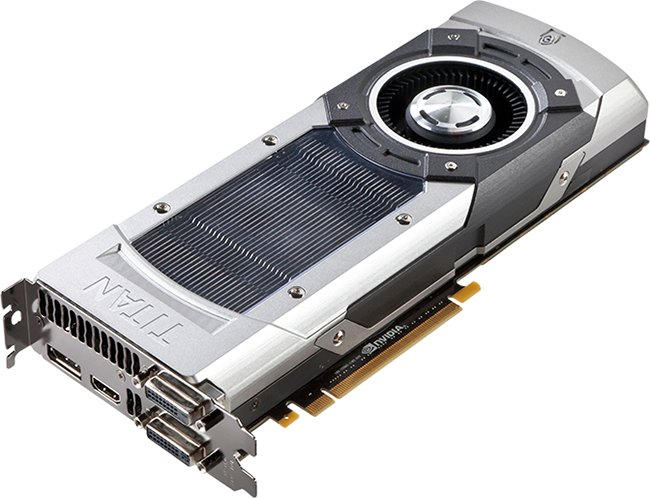
\includegraphics[width=0.8\textwidth]{img/titan}
                 \caption{NVIDIA\textsuperscript{\textregistered} GTX Titan}
                 \label{fig:titan}
             \end{figure}
        \end{column}
    \end{columns}
\end{frame}

\begin{frame}
    \frametitle{Introduction}
    \framesubtitle{CPU/GPU Design}

    \begin{itemize}
        \item CPU,
        \begin{itemize}
            \item Designed to have a good \blue{performance}
                  in parallel and non-parallel scenarios.
            \item Minimizes the \blue{latency} experimented by a thread
                  (large cache memory)
        \end{itemize}
        \item GPU,
            \begin{itemize}
            \item Designed to perform highly parallel work.
            \item Maximizes the \blue{throughput} of all the threads.
            \end{itemize}
    \end{itemize}

    \begin{footnotesize}
        \begin{columns}
            \begin{column}{0.35\textwidth}
            \begin{block}{Performance}
                Capacity of perform individual instructions in a certain time.
            \end{block}
            \end{column}
            \begin{column}{0.3\textwidth}
            \begin{block}{Latency}
                Measure of time delay experienced in a system.
            \end{block}
            \end{column}
            \begin{column}{0.3\textwidth}
            \begin{block}{Throughput}
                Capacity of perform a whole task in a certain time.
            \end{block}
            \end{column}
        \end{columns}
    \end{footnotesize}

    %\begin{description}
    %    \item[Performance]
    %            Capacity of perform individual instructions in a certain time.
    %    \item[Throughput]
    %            Capacity of perform a whole task in a certain time.
    %    \item[Latency]
    %            Measure of time delay experienced in a system.
    %    \item[Granularity]
    %            Break down a system into small parts.(Coarse and Fine)
    %\end{description}
\end{frame}

\begin{frame}
    \framesubtitle{Introduction}
    \frametitle{GPU Architecture}

    \begin{columns}
        \begin{column}{0.5\textwidth}
            \begin{block}{Task parallelism}
                Each processor perform a different task.
            \end{block}
            \begin{block}{Data parallelism}
                Each processor perform the same task, but not on the same data set.
            \end{block}
        \end{column}
        \begin{column}{0.5\textwidth}
             \begin{figure}
                 \centering
                 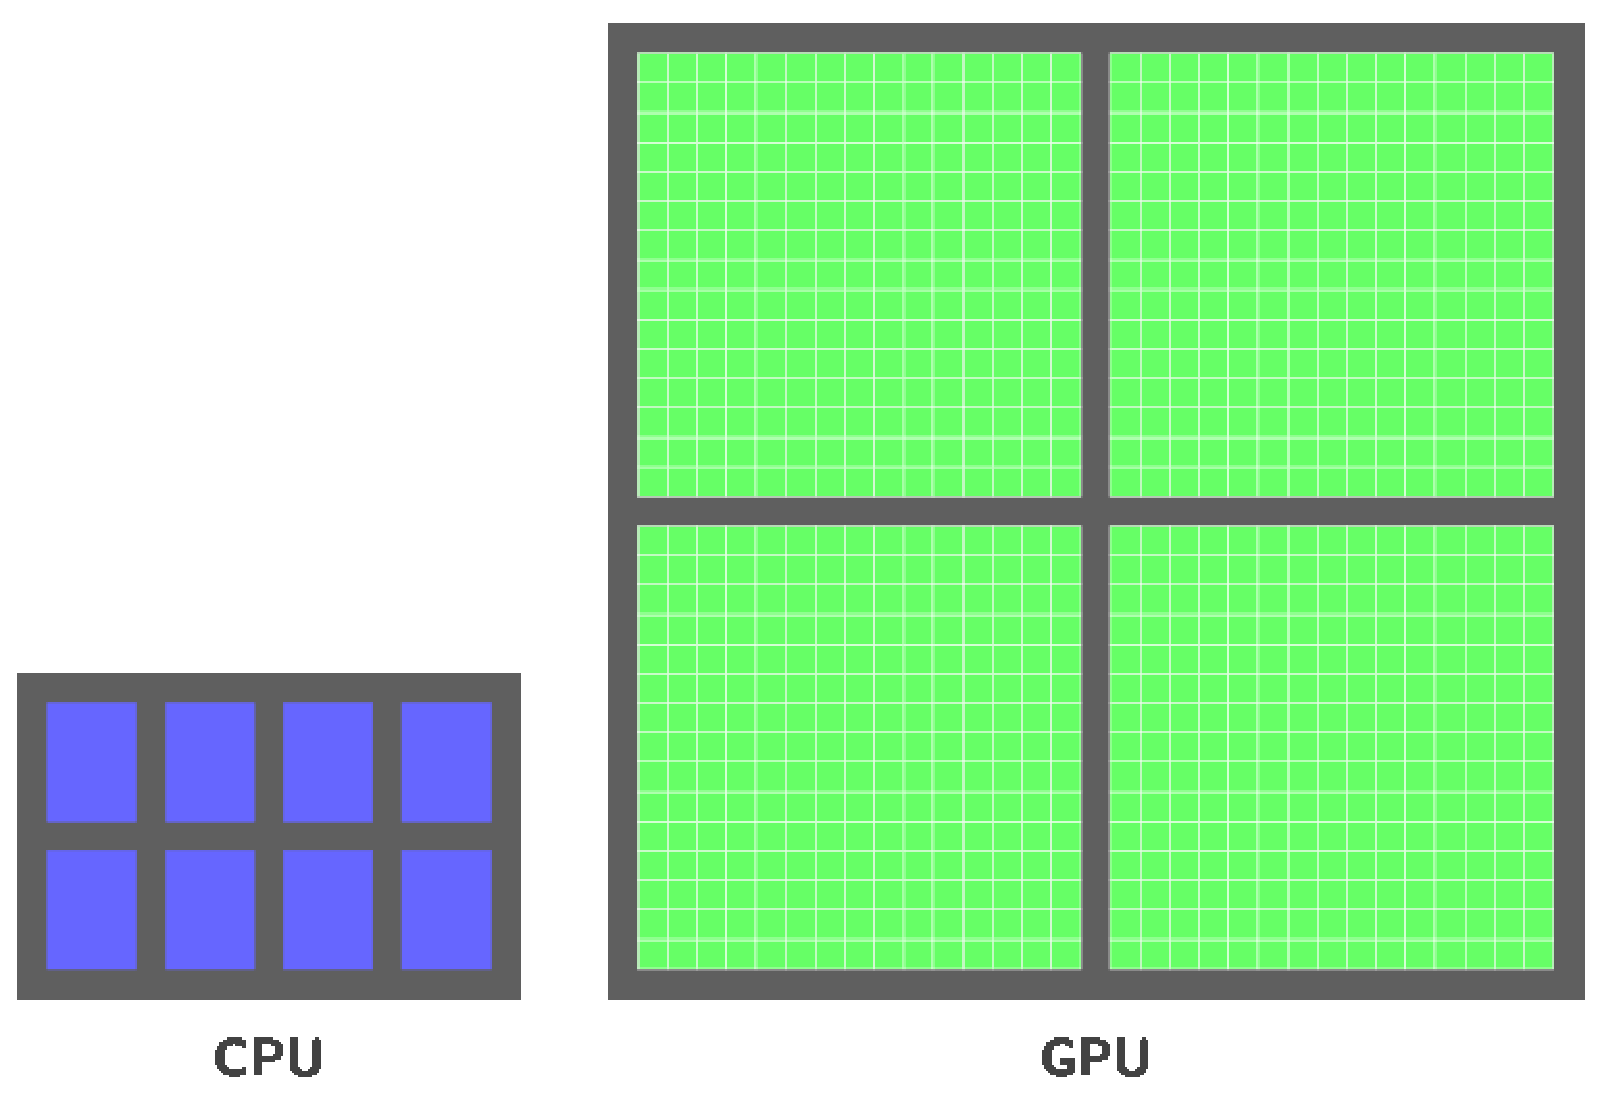
\includegraphics[width=0.8\textwidth]{img/cpu_gpu}
                 \caption{GPU and CPU core scheme}
                 \label{fig:titan}
             \end{figure}
        \end{column}
    \end{columns}
\end{frame}

\subsection{Programming strategy}
\begin{frame}
    \frametitle{Introduction}
    \framesubtitle{Programming strategy}

    \begin{columns}
        \begin{column}{0.5\textwidth}
            \begin{figure}
                \captionsetup{singlelinecheck=off}
                \centering
                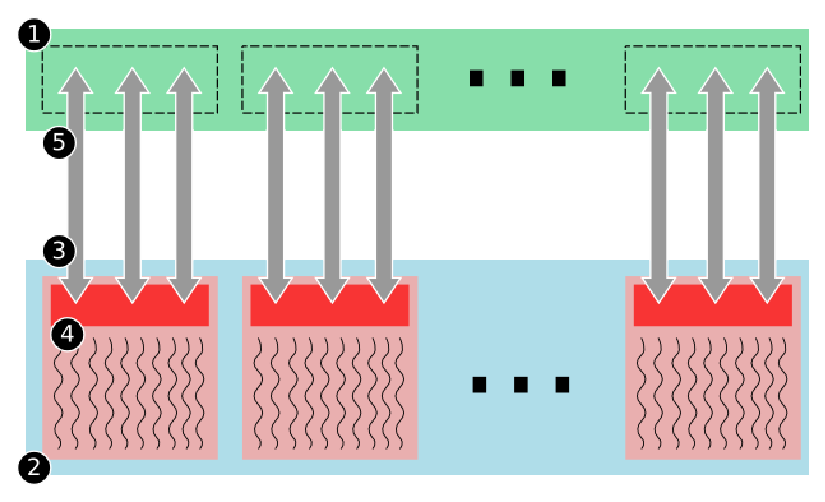
\includegraphics[width=0.9\textwidth]{img/cuda-strategy}
                \label{fig:estrategia}
                \caption{CUDA Programming strategy}
            \end{figure}
        \end{column}
        \begin{column}{0.5\textwidth}
             \begin{enumerate}
                 \item CPU memory allocation,
                 \item \dgreen{GPU} memory allocation,
                 \item Data copying,  CPU $\rightarrow$ \dgreen{GPU},
                 \item Task execution on the data,
                 \item Data copying, \dgreen{GPU} $\rightarrow$ CPU,
             \end{enumerate}
        \end{column}
    \end{columns}
\end{frame}

\begin{frame}
    \frametitle{GPU Computing}
    \framesubtitle{Introduction}

    \begin{columns}
        \begin{column}{0.5\textwidth}
            \begin{itemize}
                \item \emph{``Using a GPU (Graphic Processing Unit) together with
                      a CPU to accelerate scientific calculation operations
                      or general purpose calculation''}
            \end{itemize}
        \end{column}
        \begin{column}{0.5\textwidth}
             \begin{figure}
                 \centering
                 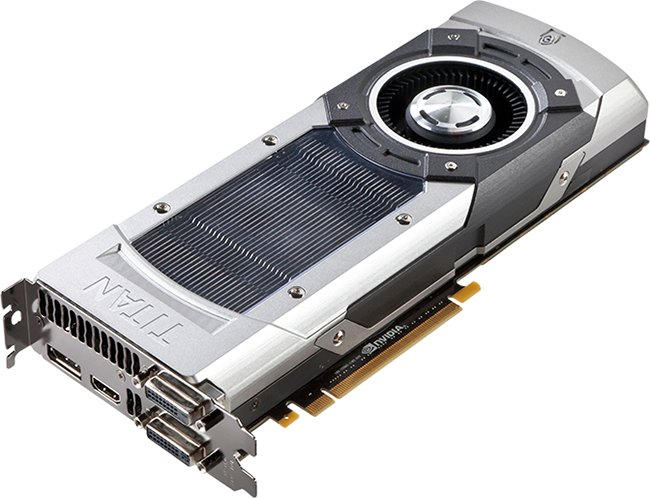
\includegraphics[width=0.8\textwidth]{img/titan}
                 \caption{NVIDIA\textsuperscript{\textregistered} GTX Titan}
                 \label{fig:titan}
             \end{figure}
        \end{column}
    \end{columns}
\end{frame}

\begin{frame}
    \frametitle{GPU Computing}
    \framesubtitle{Features}

    \begin{itemize}
        \item CPU,
        \begin{itemize}
            \item Designed to have a good \blue{performance}
                  in parallel and non-parallel scenarios.
            \item Minimizes the \blue{latency} experimented by a thread
                  (large cache memory)
        \end{itemize}
        \item GPU,
            \begin{itemize}
            \item Designed to perform highly parallel work.
            \item Maximizes the \blue{throughput} of all the threads.
            \end{itemize}
    \end{itemize}

    \begin{footnotesize}
        \begin{columns}
            \begin{column}{0.35\textwidth}
            \begin{block}{Performance}
                Capacity of perform individual instructions in a certain time.
            \end{block}
            \end{column}
            \begin{column}{0.3\textwidth}
            \begin{block}{Latency}
                Measure of time delay experienced in a system.
            \end{block}
            \end{column}
            \begin{column}{0.3\textwidth}
            \begin{block}{Throughput}
                Capacity of perform a whole task in a certain time.
            \end{block}
            \end{column}
        \end{columns}
    \end{footnotesize}

    %\begin{description}
    %    \item[Performance]
    %            Capacity of perform individual instructions in a certain time.
    %    \item[Throughput]
    %            Capacity of perform a whole task in a certain time.
    %    \item[Latency]
    %            Measure of time delay experienced in a system.
    %    \item[Granularity]
    %            Break down a system into small parts.(Coarse and Fine)
    %\end{description}
\end{frame}

\begin{frame}
    \frametitle{GPU Computing}
    \framesubtitle{Architecture}

    \begin{columns}
        \begin{column}{0.5\textwidth}
            \begin{block}{Task parallelism}
                Each processor perform a different task.
            \end{block}
            \begin{block}{Data parallelism}
                Each processor perform the same task, but not on the same data set.
            \end{block}
        \end{column}
        \begin{column}{0.5\textwidth}
             \begin{figure}
                 \centering
                 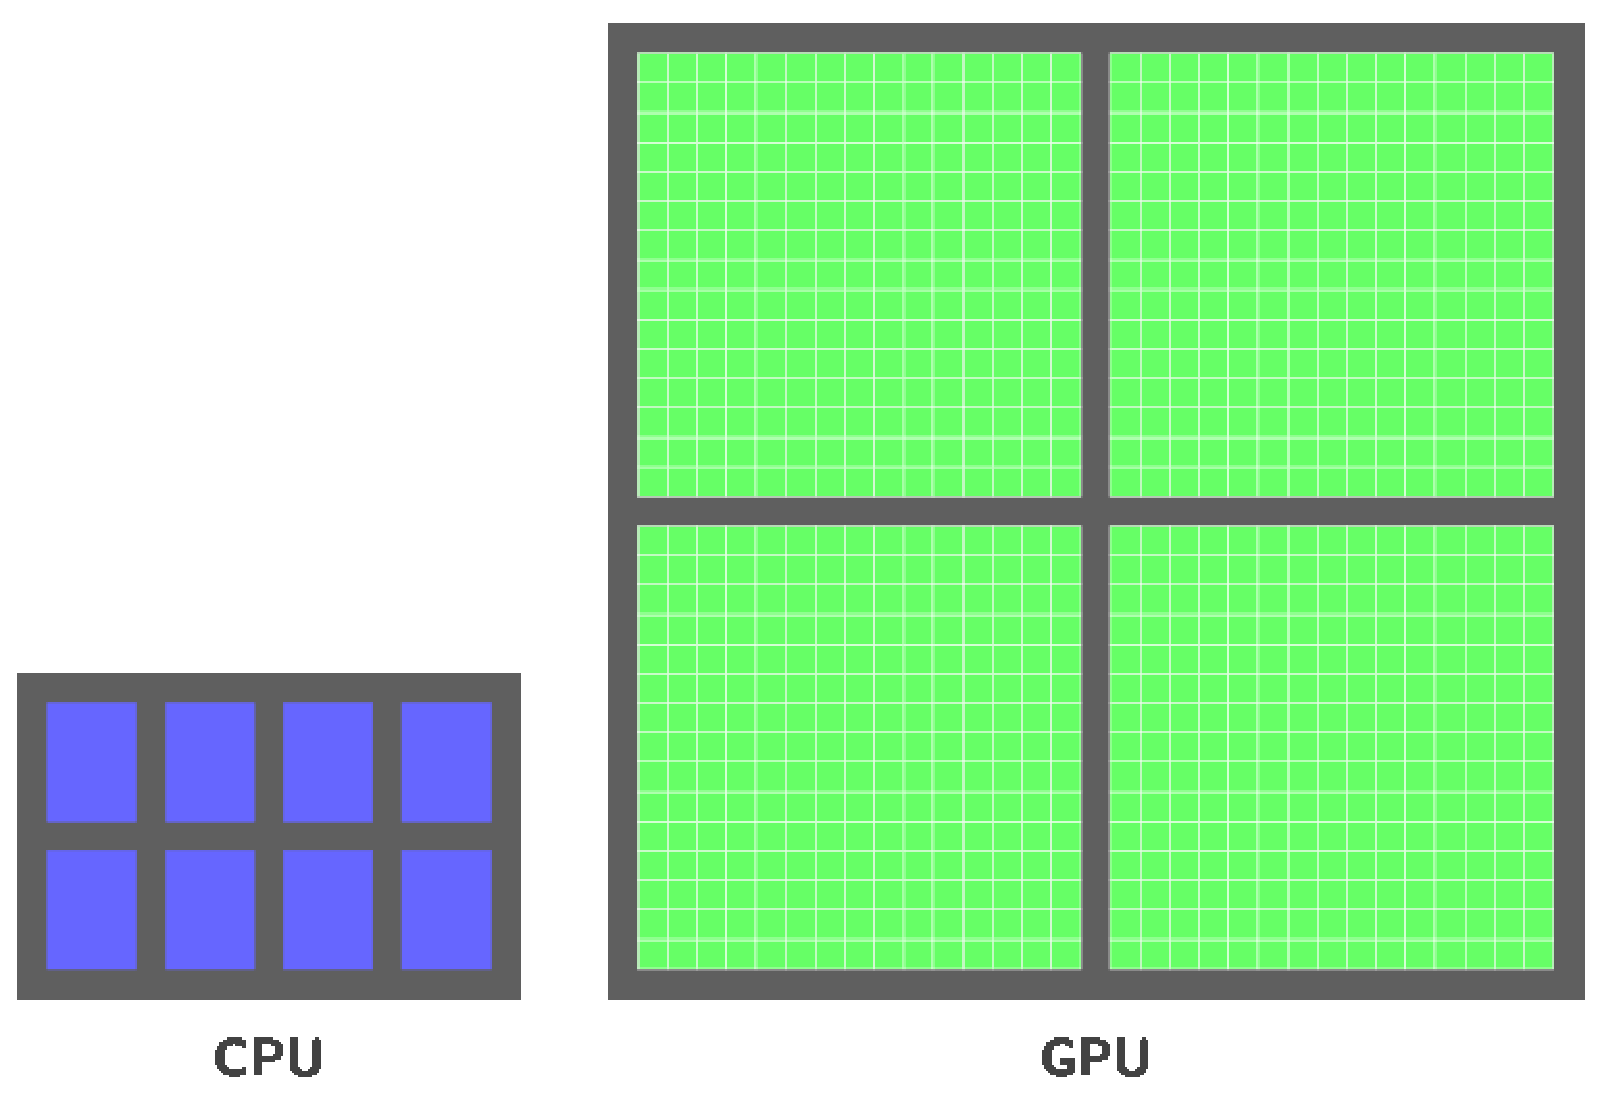
\includegraphics[width=0.8\textwidth]{img/cpu_gpu}
                 \caption{GPU and CPU core scheme}
                 \label{fig:titan}
             \end{figure}
        \end{column}
    \end{columns}
\end{frame}

\begin{frame}
    \frametitle{GPU Computing}
    \framesubtitle{Functionality}

    \begin{columns}
        \begin{column}{0.5\textwidth}
            \begin{figure}
                \captionsetup{singlelinecheck=off}
                \centering
                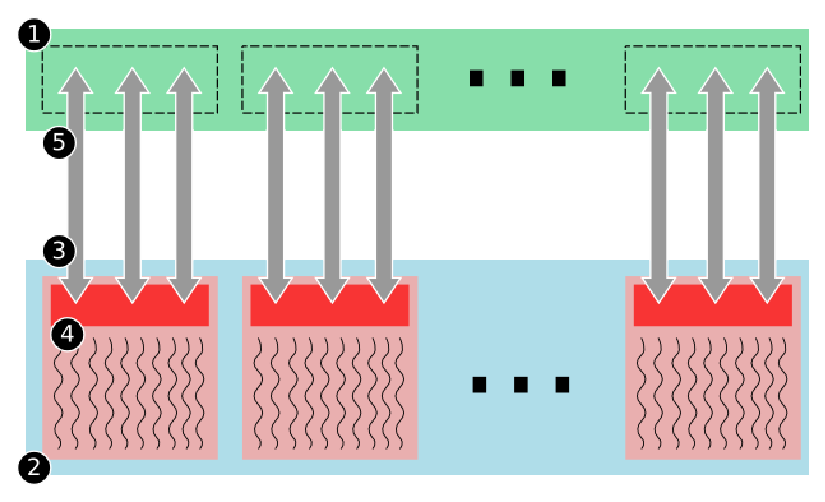
\includegraphics[width=0.9\textwidth]{img/cuda-strategy}
                \label{fig:estrategia}
                \caption{CUDA Programming strategy}
            \end{figure}
        \end{column}
        \begin{column}{0.5\textwidth}
             \begin{enumerate}
                 \item CPU memory allocation,
                 \item \dgreen{GPU} memory allocation,
                 \item Data copying,  CPU $\rightarrow$ \dgreen{GPU},
                 \item Task execution on the data,
                 \item Data copying, \dgreen{GPU} $\rightarrow$ CPU,
             \end{enumerate}
        \end{column}
    \end{columns}
\end{frame}


\documentclass{beamer}
\usepackage[english,activeacute]{babel}
\usepackage[utf8]{inputenc}
\usepackage{listings}
\usepackage{color}
\usepackage{tikz}

\definecolor{red}{RGB}{255,0,0}
\definecolor{green}{RGB}{0,255,0}
\definecolor{blue}{RGB}{0,0,255}
\definecolor{oran}{RGB}{255,93,0}

\newcommand{\blue}{\textcolor{blue}}
\newcommand{\red}{\textcolor{red}}
\newcommand{\green}{\textcolor{green}}
\newcommand{\oran}{\textcolor{oran}}
\newcommand{\gray}{\textcolor{gray}}
\definecolor{gray97}{gray}{.97}
\definecolor{gray75}{gray}{.75}
\definecolor{gray45}{gray}{.45}

\renewcommand\mathfamilydefault{\rmdefault}
\setbeamertemplate{blocks}[rounded][shadow=true]

%\usetheme[pageofpages=of,
%          alternativetitlepage=true,
%          titlepagelogo=img/aei,
%          watermark=,
%          watermarkheight=50px,
%          watermarkheightmult=1]{Torino}

\lstset{ frame=Ltb,
     framerule=0pt,
     aboveskip=0.5cm,
     framextopmargin=3pt,
     framexbottommargin=3pt,
     framexleftmargin=0.4cm,
     framesep=0pt,
     rulesep=.4pt,
     backgroundcolor=\color{gray97},
     rulesepcolor=\color{black},
     %
     stringstyle=\ttfamily,
     showstringspaces = false,
     basicstyle=\tiny\ttfamily,
     %commentstyle=\color{gray45},
     %keywordstyle=\bfseries,
     %
     numbers=left,
     numbersep=13pt,
     numberstyle=\tiny,
     numberfirstline = false,
     breaklines=true,
     emph = {[1]\_\_device\_\_,\_\_global\_\_,\_\_syncthreads,pthread\_create,pthread\_join,pragma,omp,parallel,private, threadIdx, blockDim, blockIdx,cudaThreadSynchronize, while, total},
     emphstyle={[1]\color{blue}},
   }

% minimizar fragmentado de listados
\lstnewenvironment{listing}[1][]
   {\lstset{#1}\pagebreak[0]}{\pagebreak[0]}

\lstdefinestyle{consola}
   {basicstyle=\scriptsize\bf\ttfamily,
    backgroundcolor=\color{gray75},
   }
\lstdefinestyle{C}
   {language=C,
   }



%\usecolortheme{nouvelle}
\vspace{-0.5cm}
\author[C. Maureira and P. Amaro-Seoane]
       {\large Cristián Maureira\\
        \large Pau Amaro-Seoane}
\title[GraviDy]
      {\huge \texttt{GraviDy}}
\subtitle{\large A modular direct $N$-body GPU integrator.}
\institute[AEI]
          {Albert Einstein Institute}

\begin{document}

\bibliographystyle{unsrt}
%\pagestyle{empty}

% First slide
\begin{frame}[t,plain]
    \titlepage
\end{frame}

\section{Introduction}

\begin{frame}
    \frametitle{Introduction}
    \framesubtitle{Motivation (1/2)}

    \begin{columns}
        \begin{column}{0.6\textwidth}
            \begin{itemize}
                \item Dynamical evolution of a dense stellar systems.
                      ({\nbody} Problem)
                \item Newtonian systems compounded by \blue{more than two stars},
                      needs numerical approaches.
            \end{itemize}
        \end{column}
        \begin{column}{0.4\textwidth}
            \begin{figure}
                \centering
                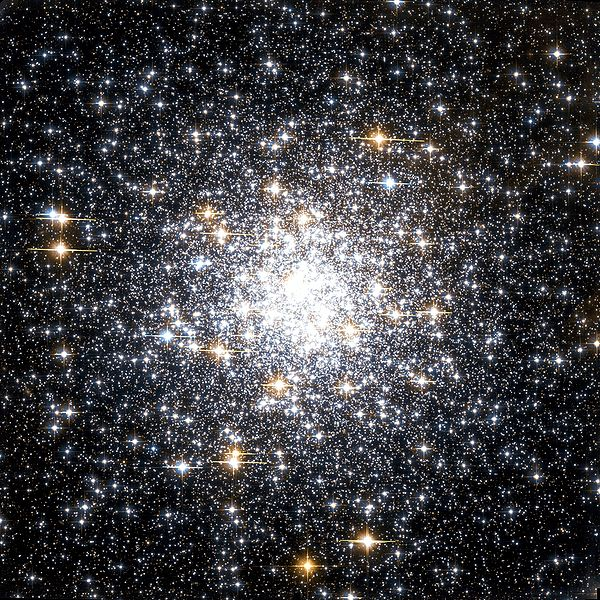
\includegraphics[width=0.8\textwidth]{img/m69}
                \caption{Globular cluster ``Messier 69'' in the constellation Sagittarius.}
                \label{fig:m69}
            \end{figure}
        \end{column}
    \end{columns}
\end{frame}

\begin{frame}
    \frametitle{Introduction}
    \framesubtitle{Motivation (2/2)}

    \begin{columns}
        \begin{column}{0.5\textwidth}
            \begin{itemize}
                \item Evolution of the High Performance Computing (HPC).
            \end{itemize}
            \begin{center}
                
\includegraphics[width=0.8\textwidth]{img/top500}
            \end{center}
        \end{column}
        \begin{column}{0.5\textwidth}
            \begin{figure}
                \centering
                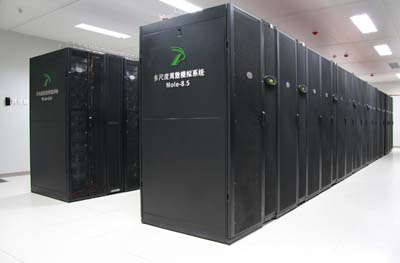
\includegraphics[width=0.8\textwidth]{img/cluster}
                \caption{GPU Cluster Mole-8.5 in Beijing, at the Institute of Process
                         Engineering of Chinese Academy of Sciences.
                         (372 nodes and 2,000 NVIDIA Fermi C2050 GPUs)}
                \label{fig:m69}
            \end{figure}
        \end{column}
    \end{columns}
\end{frame}

\section{The {\nbody} problem}
\begin{frame}
    \frametitle{The {\nbody} problem}
    \framesubtitle{Definition}

    Purely dynamic problem, in which the bodies orbital evolution
    is determined exclusive by the \blue{gravitational interaction},

    \begin{align}
        \bs{\ddot{r}}_{i} &= -G \sum\limits^{N}_{\substack{j=1\\j\neq i}}
                              m_{j} {(\bs{r}_i - \bs{r}_j)\over
                              | \bs{r}_i - \bs{r}_j|^{3}}\label{eq:nbody},
    \end{align}

    \noindent
    where $G$ is the gravitational constant
    ($6.67384\times 10^{-11} m^{3} kg^{-1} s^{-2}$),
    $m_j$ is the mass of the $j$th particle
    and $\bs{r}_j$ the position in \emph{Cartesian} coordinates.
    \begin{block}{\red{Note}}
        We denote vectors by bold fonts.
    \end{block}
\end{frame}


\begin{frame}
    \frametitle{The {\nbody} problem}
    \framesubtitle{Checking the system evolution}

    \begin{itemize}
        \item The \blue{initial condition} are usually the masses,
            position and velocity.

        \item \blue{Chaotic nature}, the evolution of this systems
         will depend of the initial parameters.

        \item The often invariant to check the integration of the system,
            is the system's \blue{energy},

            \begin{align}
                E &= {1 \over 2} \sum\limits^{N}_{i=1} m_{i} \bs{v}_{i}^{2} -
                     \sum\limits_{i=1}^{N} \sum\limits_{j > i}^{N}
                     {G m_{i} m_{j} \over |\bs{r}_{i} - \bs{r}_{j}|},
            \end{align}

            \noindent
            where $\bs{v}_i$ is the velocity of the particle $i$.
    \end{itemize}

\end{frame}


\begin{frame}
    \frametitle{The {\nbody} problem}
    \framesubtitle{Particle's time steps}

    \begin{itemize}
        \item The real scenario, \blue{individual} time steps.
        \begin{itemize}
            \item \red{Hard} scenario for parallel computing.
        \end{itemize}
        \item Forming groups of particles, \blue{block} time steps scheme~\cite{Press86}.
        \begin{itemize}
            \item  This time step scheme is popular among  {\nbody} code,
                like Starlab~\cite{portegies2001, hut2003}, Aarseth {\nbody}
                codes~\cite{Aarseth99, Aarseth03,NitadoriAarseth2012},
                $\phi$GRAPE~\cite{harfst2008},
                which gives us the possibility to check our algorithm behavior.
        \end{itemize}
    \end{itemize}
\end{frame}


\begin{frame}
    \frametitle{Introduction}
    \framesubtitle{{\nbody} algorithms classification}

    \begin{description}
        \item[Collision-less]
            A star just sees the \blue{background potential} of the rest of
            the stellar system.
            A model of this situation is the Barnes-Hut Treecode
            with a complexity $O(N\log N)$~\cite{BarnesHut86}
            or the fast multipole method with $O(N)$~\cite{GreendardThesis}.
            \vspace{0.7cm}
        \item[Collisional (``direct-summation'')]
            One star integrates \blue{all gravitational forces}
            for all stars. This typically scale as $O(N^{2})$.
            A well-known example is the family of algorithm of Aarseth
            the direct-summation {\sc Nbody} integrator~\cite{Aarseth99,Spurzem1999,Aarseth03}
            or {\sc kira} code~\cite{PortegiesZwartEtAl01}.
    \end{description}

\end{frame}

\section{Computational aspects}
\begin{frame}
    \frametitle{Introduction}
    \framesubtitle{The computational challenge}

    \begin{itemize}
        \item The {\nbody} codes evolution is related to the available
                \blue{hardware} in our time.
        \item The algorithms with a complexity of $O(N^{2})$ or $O(N^{3})$ require
                \red{supercomputers}.
        \begin{itemize}
            \item  e.g \blue{beowulf clusters},
                which require a parallelization of the code
                ({\sc Nbody6++} developed by Spurzem et al.~\cite{Spurzem1999}).

            \item Special-purpose hardware, like the \blue{GRAPE} (short for GRAvity
                PipE system~\cite{TMFES96,MT98,Makino98,GRAPE6A}.

        \end{itemize}

        \item  The literature overview reveals a strong interest on porting the existing codes to the
            \blue{GPU} architecture, like e.g. the work
            of~\cite{Portegies2007a,Hamada2007,Belleman2008}
            on single nodes or using large
            clusters~\cite{berczik2011high,NitadoriAarseth2012,Capuzzo-DolcettaEtAl2013}.

    \end{itemize}

\end{frame}

\subsection{GPU Computing}
\begin{frame}
    \frametitle{Introduction}
    \framesubtitle{GPU Computing}

    \begin{columns}
        \begin{column}{0.6\textwidth}
            \begin{itemize}
                \item \emph{``Using a GPU (Graphic Processing Unit) together with
                      a CPU to accelerate scientific calculation operations
                      or general purpose calculation''}
            \end{itemize}
        \end{column}
        \begin{column}{0.4\textwidth}
             \begin{figure}
                 \centering
                 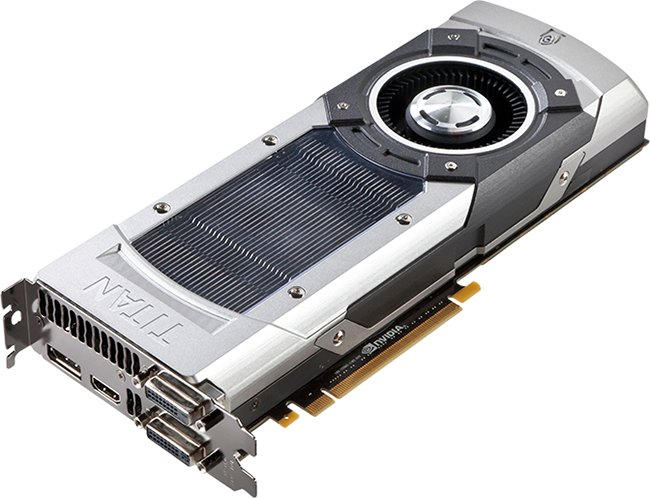
\includegraphics[width=0.8\textwidth]{img/titan}
                 \caption{NVIDIA\textsuperscript{\textregistered} GTX Titan}
                 \label{fig:titan}
             \end{figure}
        \end{column}
    \end{columns}
\end{frame}

\begin{frame}
    \frametitle{Introduction}
    \framesubtitle{CPU/GPU Design}

    \begin{itemize}
        \item CPU,
        \begin{itemize}
            \item Designed to have a good \blue{performance}
                  in parallel and non-parallel scenarios.
            \item Minimizes the \blue{latency} experimented by a thread
                  (large cache memory)
        \end{itemize}
        \item GPU,
            \begin{itemize}
            \item Designed to perform highly parallel work.
            \item Maximizes the \blue{throughput} of all the threads.
            \end{itemize}
    \end{itemize}

    \begin{footnotesize}
        \begin{columns}
            \begin{column}{0.35\textwidth}
            \begin{block}{Performance}
                Capacity of perform individual instructions in a certain time.
            \end{block}
            \end{column}
            \begin{column}{0.3\textwidth}
            \begin{block}{Latency}
                Measure of time delay experienced in a system.
            \end{block}
            \end{column}
            \begin{column}{0.3\textwidth}
            \begin{block}{Throughput}
                Capacity of perform a whole task in a certain time.
            \end{block}
            \end{column}
        \end{columns}
    \end{footnotesize}

    %\begin{description}
    %    \item[Performance]
    %            Capacity of perform individual instructions in a certain time.
    %    \item[Throughput]
    %            Capacity of perform a whole task in a certain time.
    %    \item[Latency]
    %            Measure of time delay experienced in a system.
    %    \item[Granularity]
    %            Break down a system into small parts.(Coarse and Fine)
    %\end{description}
\end{frame}

\begin{frame}
    \framesubtitle{Introduction}
    \frametitle{GPU Architecture}

    \begin{columns}
        \begin{column}{0.5\textwidth}
            \begin{block}{Task parallelism}
                Each processor perform a different task.
            \end{block}
            \begin{block}{Data parallelism}
                Each processor perform the same task, but not on the same data set.
            \end{block}
        \end{column}
        \begin{column}{0.5\textwidth}
             \begin{figure}
                 \centering
                 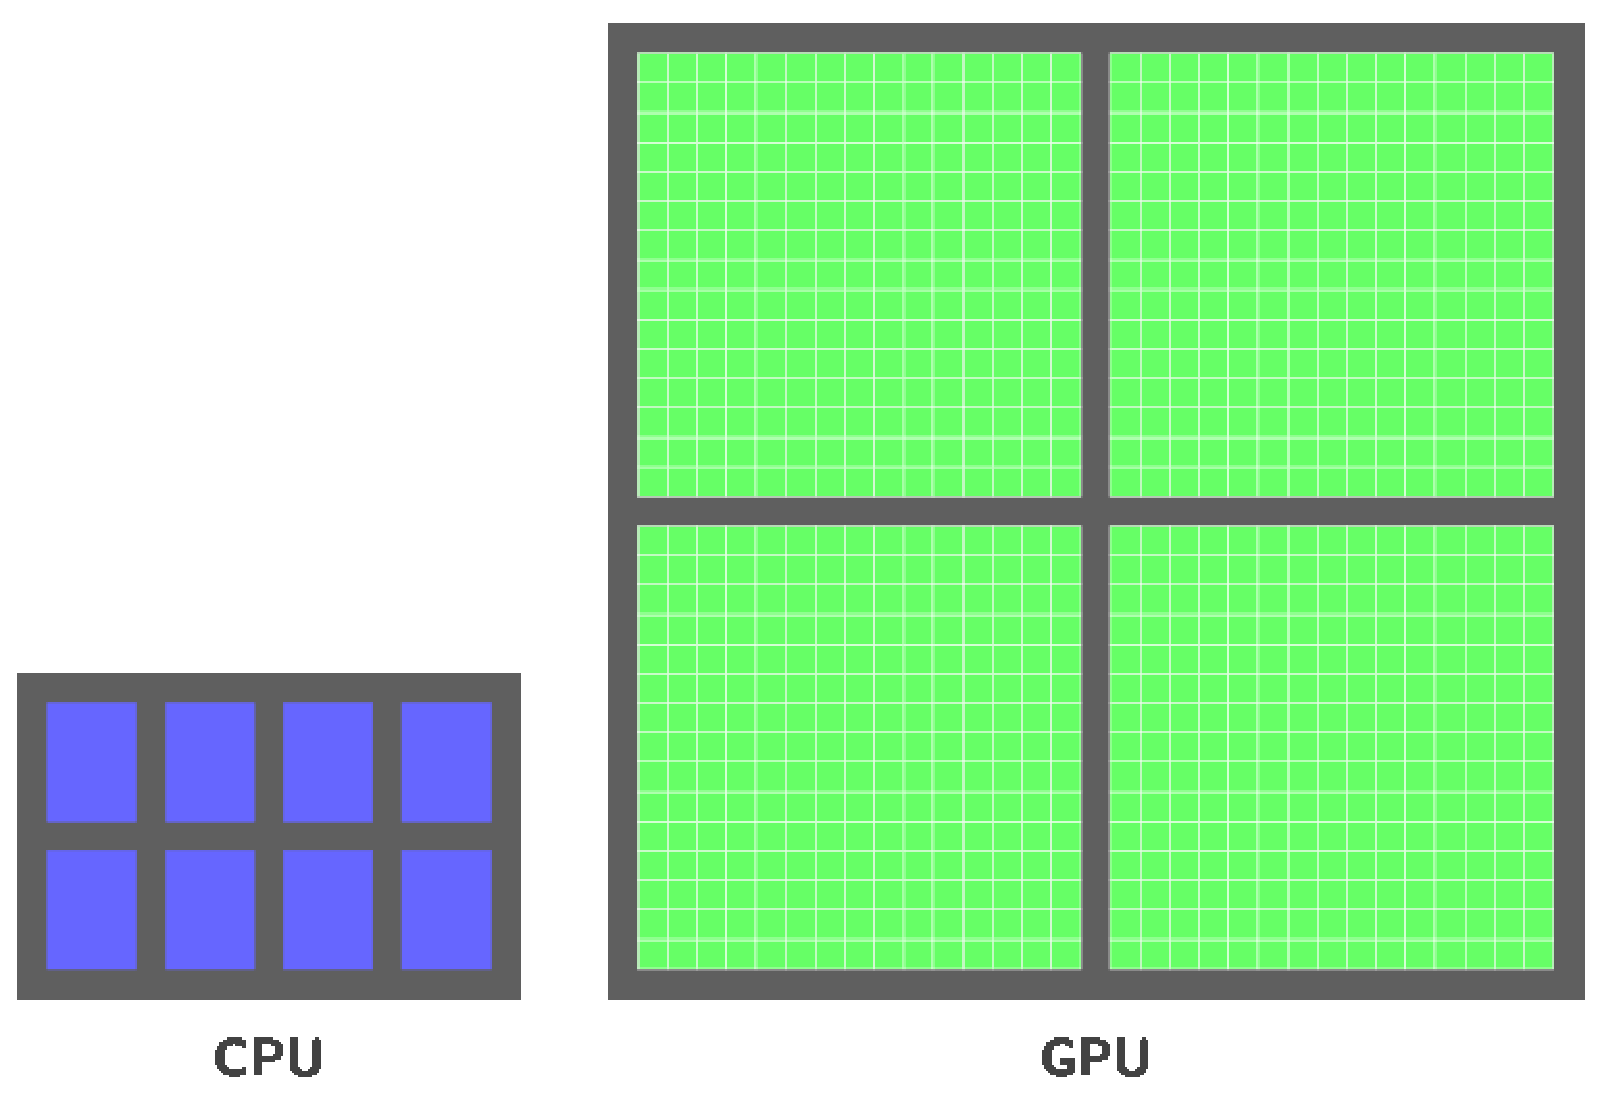
\includegraphics[width=0.8\textwidth]{img/cpu_gpu}
                 \caption{GPU and CPU core scheme}
                 \label{fig:titan}
             \end{figure}
        \end{column}
    \end{columns}
\end{frame}

\subsection{Programming strategy}
\begin{frame}
    \frametitle{Introduction}
    \framesubtitle{Programming strategy}

    \begin{columns}
        \begin{column}{0.5\textwidth}
            \begin{figure}
                \captionsetup{singlelinecheck=off}
                \centering
                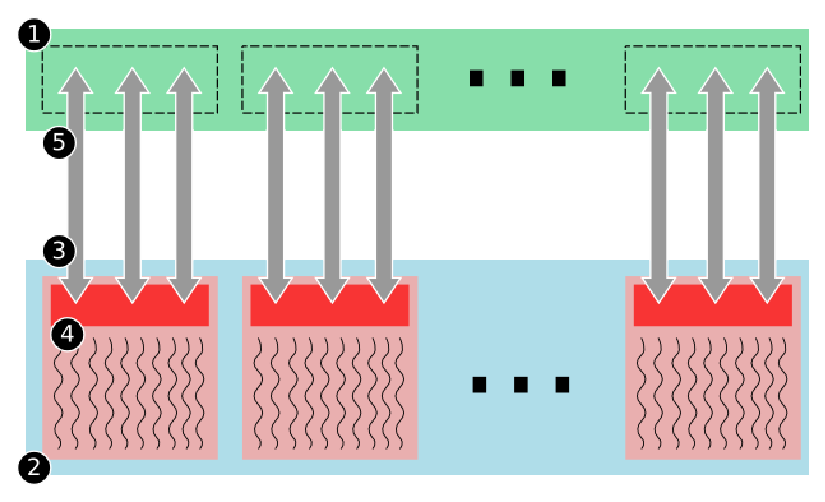
\includegraphics[width=0.9\textwidth]{img/cuda-strategy}
                \label{fig:estrategia}
                \caption{CUDA Programming strategy}
            \end{figure}
        \end{column}
        \begin{column}{0.5\textwidth}
             \begin{enumerate}
                 \item CPU memory allocation,
                 \item \dgreen{GPU} memory allocation,
                 \item Data copying,  CPU $\rightarrow$ \dgreen{GPU},
                 \item Task execution on the data,
                 \item Data copying, \dgreen{GPU} $\rightarrow$ CPU,
             \end{enumerate}
        \end{column}
    \end{columns}
\end{frame}

\begin{frame}
    \frametitle{GPU Computing}
    \framesubtitle{Introduction}

    \begin{columns}
        \begin{column}{0.5\textwidth}
            \begin{itemize}
                \item \emph{``Using a GPU (Graphic Processing Unit) together with
                      a CPU to accelerate scientific calculation operations
                      or general purpose calculation''}
            \end{itemize}
        \end{column}
        \begin{column}{0.5\textwidth}
             \begin{figure}
                 \centering
                 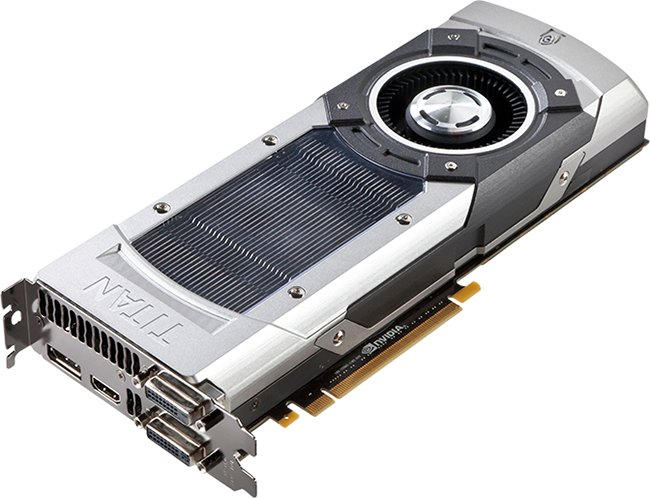
\includegraphics[width=0.8\textwidth]{img/titan}
                 \caption{NVIDIA\textsuperscript{\textregistered} GTX Titan}
                 \label{fig:titan}
             \end{figure}
        \end{column}
    \end{columns}
\end{frame}

\begin{frame}
    \frametitle{GPU Computing}
    \framesubtitle{Features}

    \begin{itemize}
        \item CPU,
        \begin{itemize}
            \item Designed to have a good \blue{performance}
                  in parallel and non-parallel scenarios.
            \item Minimizes the \blue{latency} experimented by a thread
                  (large cache memory)
        \end{itemize}
        \item GPU,
            \begin{itemize}
            \item Designed to perform highly parallel work.
            \item Maximizes the \blue{throughput} of all the threads.
            \end{itemize}
    \end{itemize}

    \begin{footnotesize}
        \begin{columns}
            \begin{column}{0.35\textwidth}
            \begin{block}{Performance}
                Capacity of perform individual instructions in a certain time.
            \end{block}
            \end{column}
            \begin{column}{0.3\textwidth}
            \begin{block}{Latency}
                Measure of time delay experienced in a system.
            \end{block}
            \end{column}
            \begin{column}{0.3\textwidth}
            \begin{block}{Throughput}
                Capacity of perform a whole task in a certain time.
            \end{block}
            \end{column}
        \end{columns}
    \end{footnotesize}

    %\begin{description}
    %    \item[Performance]
    %            Capacity of perform individual instructions in a certain time.
    %    \item[Throughput]
    %            Capacity of perform a whole task in a certain time.
    %    \item[Latency]
    %            Measure of time delay experienced in a system.
    %    \item[Granularity]
    %            Break down a system into small parts.(Coarse and Fine)
    %\end{description}
\end{frame}

\begin{frame}
    \frametitle{GPU Computing}
    \framesubtitle{Architecture}

    \begin{columns}
        \begin{column}{0.5\textwidth}
            \begin{block}{Task parallelism}
                Each processor perform a different task.
            \end{block}
            \begin{block}{Data parallelism}
                Each processor perform the same task, but not on the same data set.
            \end{block}
        \end{column}
        \begin{column}{0.5\textwidth}
             \begin{figure}
                 \centering
                 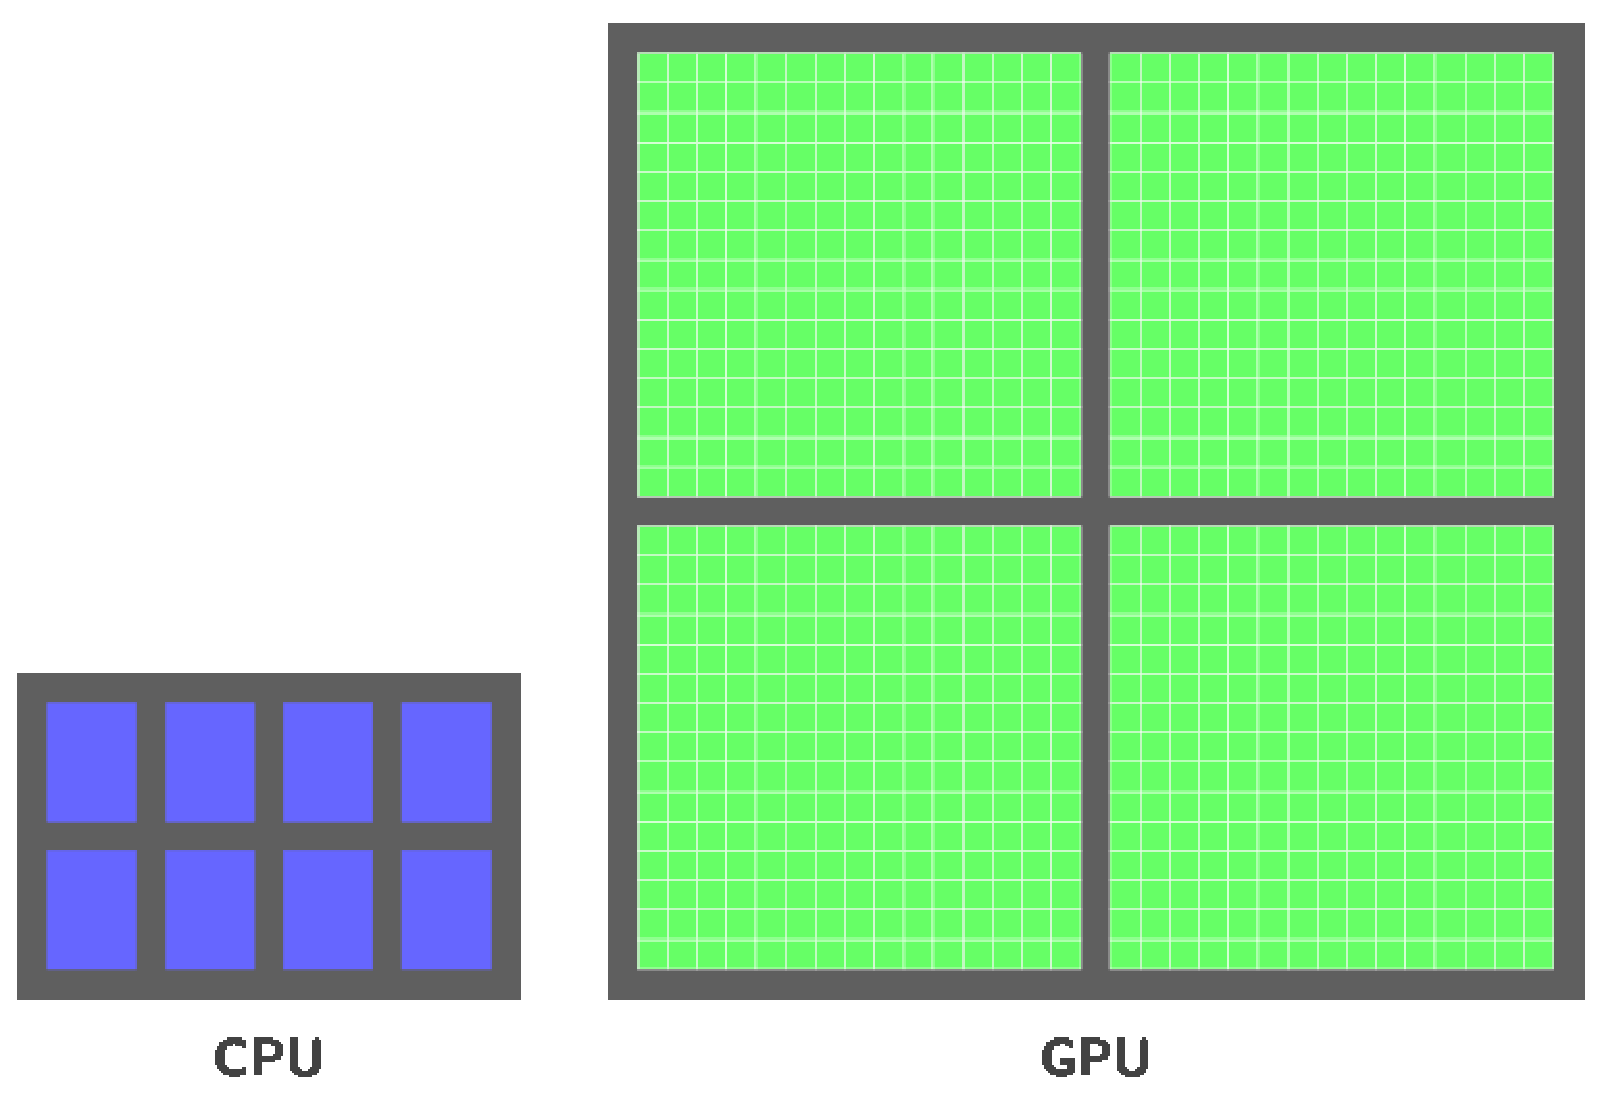
\includegraphics[width=0.8\textwidth]{img/cpu_gpu}
                 \caption{GPU and CPU core scheme}
                 \label{fig:titan}
             \end{figure}
        \end{column}
    \end{columns}
\end{frame}

\begin{frame}
    \frametitle{GPU Computing}
    \framesubtitle{Functionality}

    \begin{columns}
        \begin{column}{0.5\textwidth}
            \begin{figure}
                \captionsetup{singlelinecheck=off}
                \centering
                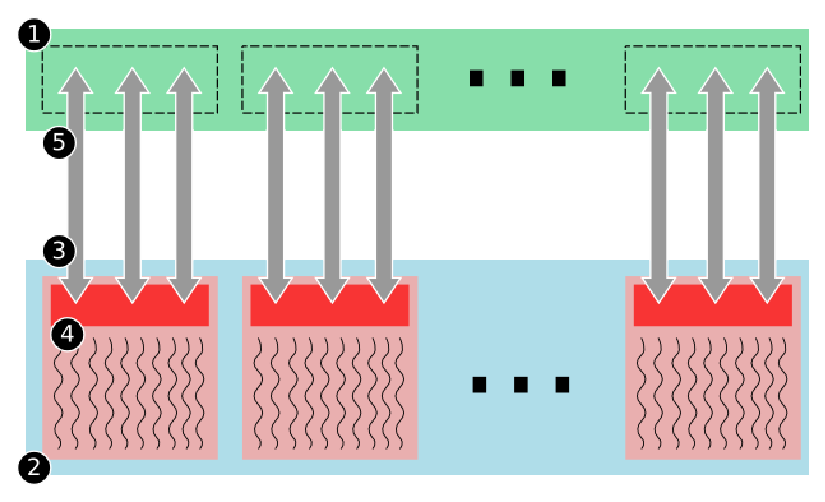
\includegraphics[width=0.9\textwidth]{img/cuda-strategy}
                \label{fig:estrategia}
                \caption{CUDA Programming strategy}
            \end{figure}
        \end{column}
        \begin{column}{0.5\textwidth}
             \begin{enumerate}
                 \item CPU memory allocation,
                 \item \dgreen{GPU} memory allocation,
                 \item Data copying,  CPU $\rightarrow$ \dgreen{GPU},
                 \item Task execution on the data,
                 \item Data copying, \dgreen{GPU} $\rightarrow$ CPU,
             \end{enumerate}
        \end{column}
    \end{columns}
\end{frame}


\documentclass{beamer}
\usepackage[english,activeacute]{babel}
\usepackage[utf8]{inputenc}
\usepackage{listings}
\usepackage{color}
\usepackage{tikz}

\definecolor{red}{RGB}{255,0,0}
\definecolor{green}{RGB}{0,255,0}
\definecolor{blue}{RGB}{0,0,255}
\definecolor{oran}{RGB}{255,93,0}

\newcommand{\blue}{\textcolor{blue}}
\newcommand{\red}{\textcolor{red}}
\newcommand{\green}{\textcolor{green}}
\newcommand{\oran}{\textcolor{oran}}
\newcommand{\gray}{\textcolor{gray}}
\definecolor{gray97}{gray}{.97}
\definecolor{gray75}{gray}{.75}
\definecolor{gray45}{gray}{.45}

\renewcommand\mathfamilydefault{\rmdefault}
\setbeamertemplate{blocks}[rounded][shadow=true]

%\usetheme[pageofpages=of,
%          alternativetitlepage=true,
%          titlepagelogo=img/aei,
%          watermark=,
%          watermarkheight=50px,
%          watermarkheightmult=1]{Torino}

\lstset{ frame=Ltb,
     framerule=0pt,
     aboveskip=0.5cm,
     framextopmargin=3pt,
     framexbottommargin=3pt,
     framexleftmargin=0.4cm,
     framesep=0pt,
     rulesep=.4pt,
     backgroundcolor=\color{gray97},
     rulesepcolor=\color{black},
     %
     stringstyle=\ttfamily,
     showstringspaces = false,
     basicstyle=\tiny\ttfamily,
     %commentstyle=\color{gray45},
     %keywordstyle=\bfseries,
     %
     numbers=left,
     numbersep=13pt,
     numberstyle=\tiny,
     numberfirstline = false,
     breaklines=true,
     emph = {[1]\_\_device\_\_,\_\_global\_\_,\_\_syncthreads,pthread\_create,pthread\_join,pragma,omp,parallel,private, threadIdx, blockDim, blockIdx,cudaThreadSynchronize, while, total},
     emphstyle={[1]\color{blue}},
   }

% minimizar fragmentado de listados
\lstnewenvironment{listing}[1][]
   {\lstset{#1}\pagebreak[0]}{\pagebreak[0]}

\lstdefinestyle{consola}
   {basicstyle=\scriptsize\bf\ttfamily,
    backgroundcolor=\color{gray75},
   }
\lstdefinestyle{C}
   {language=C,
   }



%\usecolortheme{nouvelle}
\vspace{-0.5cm}
\author[C. Maureira and P. Amaro-Seoane]
       {\large Cristián Maureira\\
        \large Pau Amaro-Seoane}
\title[GraviDy]
      {\huge \texttt{GraviDy}}
\subtitle{\large A modular direct $N$-body GPU integrator.}
\institute[AEI]
          {Albert Einstein Institute}

\begin{document}

\bibliographystyle{unsrt}
%\pagestyle{empty}

% First slide
\begin{frame}[t,plain]
    \titlepage
\end{frame}

\include{src/introduction}
\include{src/gpu}
\include{src/gravidy}
\include{src/future_work}
%\include{src/cuda}
%\include{src/thrust}

% Final slide
\begin{frame}[t,plain]
\titlepage
\end{frame}

\begin{frame}[fragile]
\scriptsize
\bibliography{gravidy}
\end{frame}

\end{document}

\begin{frame}
    \frametitle{Conclusions and Future Work}

    \begin{itemize}
        \item Writing \texttt{GraviDy} from scratch $\left(\sim 3\ months\right)$
        \item We are implementing more than one HPC technique.
            (CUDA, OpenMP, and maybe more)
        \item GraviDy is still on development and we are planning
            to add new features, like:
        \begin{itemize}
            \item KS-regularization.
            \item Neighbors sphere treatment
            \item Geodetic implementation of EMRIs
            \item Coupling with SPH stellar collisions
            \item etc.
        \end{itemize}
    \end{itemize}
\end{frame}

\begin{frame}
    \frametitle{Conclusions and Future Work}
    \begin{itemize}
        \item The code will be available on the AEI website.
        \item Under the BSD license.
        \item This collaborative work will be \red{public}.
    \end{itemize}
\end{frame}

%\include{src/cuda}
%\include{src/thrust}

% Final slide
\begin{frame}[t,plain]
\titlepage
\end{frame}

\begin{frame}[fragile]
\scriptsize
\bibliography{gravidy}
\end{frame}

\end{document}

\begin{frame}
    \frametitle{Conclusions and Future Work}

    \begin{itemize}
        \item Writing \texttt{GraviDy} from scratch $\left(\sim 3\ months\right)$
        \item We are implementing more than one HPC technique.
            (CUDA, OpenMP, and maybe more)
        \item GraviDy is still on development and we are planning
            to add new features, like:
        \begin{itemize}
            \item KS-regularization.
            \item Neighbors sphere treatment
            \item Geodetic implementation of EMRIs
            \item Coupling with SPH stellar collisions
            \item etc.
        \end{itemize}
    \end{itemize}
\end{frame}

\begin{frame}
    \frametitle{Conclusions and Future Work}
    \begin{itemize}
        \item The code will be available on the AEI website.
        \item Under the BSD license.
        \item This collaborative work will be \red{public}.
    \end{itemize}
\end{frame}

%\include{src/cuda}
%\include{src/thrust}

% Final slide
\begin{frame}[t,plain]
\titlepage
\end{frame}

\begin{frame}[fragile]
\scriptsize
\bibliography{gravidy}
\end{frame}

\end{document}

\begin{frame}
    \frametitle{Conclusions and Future Work}

    \begin{itemize}
        \item Writing \texttt{GraviDy} from scratch $\left(\sim 3\ months\right)$
        \item We are implementing more than one HPC technique.
            (CUDA, OpenMP, and maybe more)
        \item GraviDy is still on development and we are planning
            to add new features, like:
        \begin{itemize}
            \item KS-regularization.
            \item Neighbors sphere treatment
            \item Geodetic implementation of EMRIs
            \item Coupling with SPH stellar collisions
            \item etc.
        \end{itemize}
    \end{itemize}
\end{frame}

\begin{frame}
    \frametitle{Conclusions and Future Work}
    \begin{itemize}
        \item The code will be available on the AEI website.
        \item Under the BSD license.
        \item This collaborative work will be \red{public}.
    \end{itemize}
\end{frame}

%\include{src/cuda}
%\include{src/thrust}

% Final slide
\begin{frame}[t,plain]
\titlepage
\end{frame}

\begin{frame}[fragile]
\scriptsize
\bibliography{gravidy}
\end{frame}

\end{document}
